\documentclass[11pt]{report}

\usepackage[margin=1in]{geometry}
\usepackage[T1]{fontenc}
\usepackage[utf8]{inputenc}
\usepackage{amsmath,amssymb,amsthm,mathtools,bm}
\let\openbox\relax
\usepackage{newpxtext,newpxmath}
\usepackage{microtype}
\usepackage{setspace}
\setstretch{1.12}
\setlength{\parskip}{0.45em}
\setlength{\parindent}{0pt}
\usepackage{booktabs,array,tabularx,longtable}
\usepackage{enumitem}
\setlist{itemsep=0.35em,topsep=0.4em}

\usepackage{tikz}
\usetikzlibrary{arrows.meta,positioning,calc,shapes.geometric,fit,backgrounds}

\usepackage[most]{tcolorbox}

\definecolor{ink}{HTML}{1C1915}
\definecolor{muted}{HTML}{5C564C}
\definecolor{paper}{HTML}{FFFFFF}
\definecolor{rule}{HTML}{E0D5C4}
\definecolor{burgundy}{HTML}{8D3B2E}
\definecolor{burgundysoft}{HTML}{F6EBE7}
\definecolor{navy}{HTML}{1F4E79}
\definecolor{navysoft}{HTML}{E7F0F7}
\definecolor{teal}{HTML}{1D6A5A}
\definecolor{tealsoft}{HTML}{E5F4EF}
\definecolor{amber}{HTML}{8A5A12}
\definecolor{ambersoft}{HTML}{FBF3E4}
\definecolor{plum}{HTML}{5C3D6E}
\definecolor{plumsoft}{HTML}{F3ECF6}
\definecolor{slate}{HTML}{3E4A59}

\pagecolor{paper}
\color{ink}

\usepackage{hyperref}
\hypersetup{
  colorlinks=true,
  linkcolor=burgundy,
  citecolor=navy,
  urlcolor=navy,
  pdftitle={Theory guide for Deep Generative Models, Homeworks 1 and 2},
  pdfauthor={Study notes for course 25732-1}
}

\newtcolorbox{defbox}[1][]{%
  breakable, enhanced, colback=navysoft, colframe=navy,
  coltitle=white, fonttitle=\bfseries, title={Definition\ifstrempty{#1}{}{: #1}},
  arc=2pt, boxrule=0.7pt, left=8pt, right=8pt, top=6pt, bottom=6pt}

\newtcolorbox{resultbox}[1][]{%
  breakable, enhanced, colback=burgundysoft, colframe=burgundy,
  coltitle=white, fonttitle=\bfseries, title={Result\ifstrempty{#1}{}{: #1}},
  arc=2pt, boxrule=0.7pt, left=8pt, right=8pt, top=6pt, bottom=6pt}

\newtcolorbox{intbox}[1][]{%
  breakable, enhanced, colback=tealsoft, colframe=teal,
  coltitle=white, fonttitle=\bfseries, title={Intuition\ifstrempty{#1}{}{: #1}},
  arc=2pt, boxrule=0.7pt, left=8pt, right=8pt, top=6pt, bottom=6pt}

\newtcolorbox{practbox}[1][]{%
  breakable, enhanced, colback=ambersoft, colframe=amber,
  coltitle=white, fonttitle=\bfseries, title={Practice\ifstrempty{#1}{}{: #1}},
  arc=2pt, boxrule=0.7pt, left=8pt, right=8pt, top=6pt, bottom=6pt}

\newtcolorbox{solbox}[1][]{%
  breakable, enhanced, colback=plumsoft, colframe=plum,
  coltitle=white, fonttitle=\bfseries, title={Worked solution\ifstrempty{#1}{}{: #1}},
  arc=2pt, boxrule=0.7pt, left=8pt, right=8pt, top=6pt, bottom=6pt}

\newtcolorbox{pitbox}[1][]{%
  breakable, enhanced, colback=white, colframe=burgundy,
  coltitle=burgundy, fonttitle=\bfseries, title={Watch out\ifstrempty{#1}{}{: #1}},
  arc=2pt, boxrule=0.8pt, left=8pt, right=8pt, top=6pt, bottom=6pt,
  borderline west={3pt}{0pt}{burgundy}}

\newtcolorbox{hwqbox}[1][]{%
  breakable, enhanced, colback=ambersoft, colframe=amber,
  coltitle=white, fonttitle=\bfseries, title={Homework question\ifstrempty{#1}{}{: #1}},
  arc=2pt, boxrule=0.7pt, left=8pt, right=8pt, top=6pt, bottom=6pt}

\newtcolorbox{hwsolbox}[1][]{%
  breakable, enhanced, colback=plumsoft, colframe=plum,
  coltitle=white, fonttitle=\bfseries, title={Homework answer\ifstrempty{#1}{}{: #1}},
  arc=2pt, boxrule=0.7pt, left=8pt, right=8pt, top=6pt, bottom=6pt}

\newcommand{\E}{\mathbb{E}}
\newcommand{\R}{\mathbb{R}}
\newcommand{\Z}{\mathbb{Z}}
\newcommand{\N}{\mathcal{N}}
\newcommand{\KL}{\mathrm{KL}}
\newcommand{\JS}{\mathrm{JS}}
\newcommand{\diag}{\operatorname{diag}}
\newcommand{\tr}{\operatorname{tr}}
\DeclareMathOperator{\logit}{logit}
\newcommand{\given}{\mid}

\title{\textcolor{burgundy}{Deep Generative Models}\\[0.4em]
\large A theory guide for Homework 1 and Homework 2}
\author{Course 25732-1 \quad Dr.\ Sajjad Amini\\
Department of Electrical Engineering\\
Sharif University of Technology}
\date{Fall 2026}

\begin{document}
\maketitle
\begin{center}
\textcolor{muted}{Lecture numbers refer to the decks in \texttt{lectures/}.\\
Slide numbers are the numbers printed on the slides.}
\end{center}
\tableofcontents

\chapter{How to use this guide}
\label{ch:map}

This note teaches the mathematics that Homeworks 1 and 2 actually use. Each chapter states a definition, gives the intuition, derives the identity, draws the picture, and then poses a short practice problem with a worked solution. The practice problems are smaller than the homework. They train the same moves.

\begin{intbox}[What to read for which homework]
Homework 1 uses Chapters~\ref{ch:prob}--\ref{ch:ar}. Homework 2 uses those chapters and then Chapters~\ref{ch:vae}--\ref{ch:flow}. The conditional ELBO, the hierarchical ELBO, dequantization, and the Glow convolution are extensions of the lectures. Their derivations are written out here.
\end{intbox}

\begin{center}
\renewcommand{\arraystretch}{1.25}
\begin{tabularx}{\textwidth}{@{}lXl@{}}
\toprule
\textbf{Homework piece} & \textbf{Read} & \textbf{Slides}\\
\midrule
Gaussians, products, conditionals & Ch.~\ref{ch:gauss} & L2, 12--35\\
KL, Jensen--Shannon, perplexity & Ch.~\ref{ch:info} & L2, 36--42\\
Monte Carlo, importance sampling & Ch.~\ref{ch:mc} & L2, 34--35; L4, 23--29\\
Markov models and autoregression & Ch.~\ref{ch:ar} & L3\\
ELBO, reparameterization, CVAE & Ch.~\ref{ch:vae} & L4, 12--40, 56--84\\
Two-layer hierarchical ELBO & Ch.~\ref{ch:hier} & pattern of L4, 38--39\\
Coupling, flow prior, dequantization, Glow & Ch.~\ref{ch:flow} & L5, 3--73\\
\bottomrule
\end{tabularx}
\end{center}

\begin{defbox}[Notation used throughout]
Random variables are capitals when the distinction matters, and the same letter is used for a value when the slides do so. A Gaussian $\N(x\given\mu,\sigma^2)$ has variance $\sigma^2$, matching Lecture~2. $\log$ is the natural logarithm, so information quantities are in nats. $\KL(q\Vert p)$ means we use $q$ where the reference in the denominator is $p$. The Jacobian $J_f(u)$ is the matrix of partial derivatives $\partial f_i/\partial u_j$.
\end{defbox}

\chapter{Probability}
\label{ch:prob}

\section{Events, variables, and densities}

\begin{defbox}[Density and mass]
A discrete random variable $X$ has a probability mass function $p(x)\ge 0$ with $\sum_x p(x)=1$. A continuous random variable on $\R^d$ has a density $p(x)\ge 0$ with $\int p(x)\,dx=1$. The density is not a probability. $p(x)$ can exceed $1$. The probability of a set $A$ is $\int_A p(x)\,dx$.
\end{defbox}

\begin{intbox}
Think of a density as height and a probability as area. A very narrow bump can be very tall and still have area one. This is why, later, the flow density $p_\theta(x)$ at an integer pixel is not the probability of that pixel.
\end{intbox}

The joint density $p(x,z)$ describes the pair. The marginal of $x$ sums or integrates the other variable out,
\[
p(x)=\int p(x,z)\,dz.
\]
The conditional is the joint divided by the marginal, when the marginal is positive:
\[
p(z\given x)=\frac{p(x,z)}{p(x)},\qquad p(x,z)=p(x\given z)\,p(z).
\]
The second display is the chain rule. It is the only legal way to build a joint from conditionals on a directed graph: each node is conditioned on its parents, and the graph is acyclic.

\begin{resultbox}[Bayes]
\[
p(z\given x)=\frac{p(x\given z)\,p(z)}{p(x)}.
\]
The denominator is the marginal likelihood. In a latent-variable model it is the integral that the ELBO avoids computing.
\end{resultbox}

\section{Expectation, variance, and Jensen}

\begin{defbox}[Expectation]
For a function $f$ and a density $p$,
\[
\E_{x\sim p}[f(x)]=\int f(x)\,p(x)\,dx,
\]
when the integral exists. Linearity holds even if the coordinates of $x$ are dependent: $\E[a^\top x]=a^\top\E[x]$.
\end{defbox}

Variance is $\mathrm{Var}(f)=\E[f^2]-(\E f)^2$. For a sum of independent random variables the variances add. They do not add when the variables share randomness. That fact is the whole of the importance-sampling variance story: a bad proposal makes $f\,p/q$ wildly dependent on the draw.

\begin{resultbox}[Jensen]
If $\psi$ is concave and the expectations exist, then $\psi(\E[X])\ge \E[\psi(X)]$. The logarithm is concave, so
\[
\log \E[X]\ge \E[\log X].
\]
Equality holds when $X$ is almost surely constant, or more generally when $\psi$ is affine on the range of $X$.
\end{resultbox}

\begin{intbox}
Jensen is the reason a lower bound appears every time a logarithm moves inside an expectation. Lecture~4, slide~34, writes exactly this for $\psi=\log$. Homework~2 uses it twice: once for the ELBO, and once for variational dequantization.
\end{intbox}

\begin{practbox}[A one-line Jensen gap]
Let $Z\in\{0,1\}$ with equal probability, and let $f(0)=1$, $f(1)=e$. Compare $\log\E[f(Z)]$ with $\E[\log f(Z)]$.
\end{practbox}
\begin{solbox}
$\E[f]=(1+e)/2$, so $\log\E[f]=\log(1+e)-\log 2$. And $\E[\log f]=\tfrac12\log 1+\tfrac12\log e=\tfrac12$. The gap is $\log(1+e)-\log 2-\tfrac12>0$ because $f$ is not constant.
\end{solbox}

\chapter{Matrix calculus and Jacobians}
\label{ch:calc}

Generative models differentiate scalars with respect to vectors and matrices. This chapter fixes the conventions and derives the four derivatives the homeworks need: a linear form, a quadratic form, a log-determinant, and a Jacobian determinant.

\section{Layout}

A scalar $L(\theta)$ has a gradient $\nabla_\theta L$ that is a column vector of the same shape as $\theta$. The differential is the inner product
\[
dL=\langle \nabla_\theta L,\, d\theta\rangle.
\]
If $\theta$ is a matrix, the inner product is the Frobenius product $\langle A,B\rangle=\tr(A^\top B)$. This is the layout used below. It matches the chain rule in coordinates.

\begin{resultbox}[Linear and quadratic forms]
Let $a\in\R^d$ be constant and let $A\in\R^{d\times d}$ be constant. Then
\begin{align*}
\nabla_x (a^\top x)&=a,\\
\nabla_x (x^\top A x)&=(A+A^\top)x.
\end{align*}
If $A$ is symmetric, the second gradient is $2Ax$. In particular $\nabla_x \|x\|^2=2x$ and $\nabla_x \tfrac12\|x\|^2=x$.
\end{resultbox}

\begin{intbox}
The factor $2$ is the usual one from $(x^2)'=2x$. People drop it when they differentiate $\tfrac12 x^\top \Sigma^{-1}x$, because the $\tfrac12$ cancels the $2$. Gaussian exponents are written with that $\tfrac12$ for this reason.
\end{intbox}

\section{Trace and log-determinant}

\begin{resultbox}[Derivatives in the matrix]
For constant $B$ and invertible $A$,
\begin{align*}
\nabla_A \tr(A^\top B)&=B,\\
\nabla_A \log\lvert\det A\rvert&=A^{-\top}.
\end{align*}
The second identity is the matrix calculus behind Glow. If $W$ depends on a diagonal vector $s$ only through $W=\diag(s)$, then
\[
\frac{\partial}{\partial s_i}\log\lvert\det W\rvert=\frac{1}{s_i}
\quad\text{when }s_i\neq 0,
\]
and the gradient of $\sum_i\log\lvert s_i\rvert$ is the vector $(1/s_i)$.
\end{resultbox}

A short derivation of the log-determinant: $\det(A+dA)=\det(A)\det(I+A^{-1}dA)$, and $\det(I+H)=1+\tr(H)+o(\|H\|)$. Therefore
\[
d\log\lvert\det A\rvert=\tr(A^{-1}\,dA)=\langle A^{-\top},\, dA\rangle.
\]

\section{Jacobians and the change-of-variables factor}

Let $f:\R^D\to\R^D$ be continuously differentiable and invertible, with differentiable inverse, and with $J_f(u)$ invertible at the points we use. If $u$ has density $p_0$ and $y=f(u)$, then $y$ has density
\begin{equation}
\label{eq:cov}
p(y)=p_0(f^{-1}(y))\,\lvert\det J_{f^{-1}}(y)\rvert
=p_0(u)\,\lvert\det J_f(u)\rvert^{-1}.
\end{equation}
In logarithms, with $u=f^{-1}(y)$,
\[
\log p(y)=\log p_0(u)-\log\lvert\det J_f(u)\rvert.
\]

\begin{intbox}[Why the absolute value]
A reflection $f(u)=-u$ preserves probability but has Jacobian $-1$. Densities are nonnegative, so the volume factor is the absolute value of the determinant. On a triangular matrix the determinant is the product of the diagonal entries, which is why coupling layers are easy.
\end{intbox}

\begin{resultbox}[Triangular determinant]
If $L$ is lower triangular with ones on the diagonal, $\det L=1$. If $U$ is strictly upper triangular, then $U+\diag(s)$ is upper triangular with diagonal $s$, and $\det(U+\diag(s))=\prod_i s_i$. A permutation matrix $P$ has $\det P=\pm 1$. Hence if $W=PL(U+\diag(s))$,
\[
\log\lvert\det W\rvert=\sum_{i=1}^{C}\log\lvert s_i\rvert.
\]
\end{resultbox}

\begin{practbox}[A $2\times 2$ Jacobian]
Let $f(u_1,u_2)=(u_1,\, u_2+u_1^2)$. Compute $J_f$, its determinant, and the density of $y=f(u)$ when $u\sim\N(0,I_2)$.
\end{practbox}
\begin{solbox}
\[
J_f(u)=\begin{pmatrix}1&0\\ 2u_1&1\end{pmatrix},\qquad \det J_f=1.
\]
The map is a shear. It preserves volume, so $\log p(y)=\log p_0(f^{-1}(y))$. The inverse is $(y_1,\, y_2-y_1^2)$, and
\[
p(y)=(2\pi)^{-1}\exp\bigl(-\tfrac12 y_1^2-\tfrac12(y_2-y_1^2)^2\bigr).
\]
This is the map in Homework~2, problem~3.2. It will return there as a counterexample to a diagonal-Gaussian restriction.
\end{solbox}

\chapter{Divergences}
\label{ch:info}

\section{Kullback--Leibler divergence}

\begin{defbox}
For densities $p$ and $q$ with $q>0$ wherever $p>0$,
\[
\KL(p\Vert q)=\E_{x\sim p}\Bigl[\log\frac{p(x)}{q(x)}\Bigr]
=\int p(x)\log\frac{p(x)}{q(x)}\,dx.
\]
\end{defbox}

\begin{resultbox}[Properties from Lecture 2, slides 36--39]
\begin{enumerate}[label=\arabic*.]
\item $\KL(p\Vert q)\ge 0$.
\item $\KL(p\Vert q)=0$ if and only if $p=q$ almost everywhere.
\item $\KL(p\Vert q)\neq \KL(q\Vert p)$ in general.
\item KL is not a distance: it fails symmetry and the triangle inequality.
\item KL may be infinite when the supports disagree.
\end{enumerate}
\end{resultbox}

The proof of nonnegativity is Jensen. Write
\[
-\KL(p\Vert q)=\E_p\bigl[\log(q/p)\bigr]\le \log \E_p[q/p]=\log\int q=0,
\]
so the KL is at least zero. Equality in Jensen holds when $q/p$ is constant on the support of $p$. Normalization forces that constant to be $1$.

\begin{pitbox}[Which way the KL points]
In a VAE the bound contains $\KL(q_\phi(z\given x)\Vert p_\theta(z))$. The first argument is the encoder, the second is the prior. Pushing that KL to zero makes the encoder match the prior, which is not the same as making the prior match the aggregated encoder. The asymmetry is the source of posterior collapse and of the off-mode mass of a Gaussian prior.
\end{pitbox}

\section{Closed-form Gaussian KL}

Let $q=\N(\mu_q,\diag(\sigma_q^2))$ and $p=\N(\mu_p,\diag(\sigma_p^2))$ on $\R^d$, with every $\sigma>0$. Independence across coordinates splits the KL into a sum. In one dimension, the Gaussian density contributes
\[
\log q(z)=-\tfrac12\log(2\pi\sigma_q^2)-\frac{(z-\mu_q)^2}{2\sigma_q^2}.
\]
Taking the expectation under $q$ and subtracting the same expression for $p$ gives, after using $\E_q[(z-\mu_q)^2]=\sigma_q^2$ and $\E_q[(z-\mu_p)^2]=\sigma_q^2+(\mu_q-\mu_p)^2$,
\begin{resultbox}[Diagonal Gaussian KL]
\begin{equation}
\label{eq:diagkl}
\KL(q\Vert p)=\frac12\sum_{j=1}^{d}
\Biggl(
\log\frac{\sigma_{p,j}^2}{\sigma_{q,j}^2}
-1
+\frac{\sigma_{q,j}^2+(\mu_{q,j}-\mu_{p,j})^2}{\sigma_{p,j}^2}
\Biggr).
\end{equation}
Against the standard normal $p=\N(0,I)$ this collapses to
\begin{equation}
\label{eq:stdkl}
\KL(q\Vert \N(0,I))=\frac12\sum_{j=1}^{d}\bigl(\mu_{q,j}^2+\sigma_{q,j}^2-1-\log\sigma_{q,j}^2\bigr).
\end{equation}
\end{resultbox}

Equation~\eqref{eq:stdkl} is the KL implemented in the VAE notebook. Equation~\eqref{eq:diagkl} is Homework~2, problem~1.3, before that specialization.

The same calculation with full covariances $\Sigma_0,\Sigma_1\succ 0$ produces the multivariate formula used in Homework~1, problem~1.4(b). Write $p_i=\N(\mu_i,\Sigma_i)$. Then
\begin{resultbox}[Multivariate Gaussian KL]
\label{res:mvnkl}
\begin{equation}
\label{eq:mvnkl}
\KL(p_0\Vert p_1)
=\frac12\Biggl[
\tr(\Sigma_1^{-1}\Sigma_0)
+(\mu_0-\mu_1)^\top\Sigma_1^{-1}(\mu_0-\mu_1)
-d
+\log\frac{\det\Sigma_1}{\det\Sigma_0}
\Biggr].
\end{equation}
\end{resultbox}
The trace and Mahalanobis terms come from $\E_{p_0}[(x-\mu_1)^\top\Sigma_1^{-1}(x-\mu_1)]$. Subtracting the differential entropy $h(p_0)=\tfrac d2\log(2\pi e)+\tfrac12\log\det\Sigma_0$ cancels the $\tfrac d2\log(2\pi)$ pieces and leaves~\eqref{eq:mvnkl}. Chapter~\ref{ch:gauss} uses this formula inside the maximum-entropy Pythagorean identity.

\begin{practbox}[A number you can check by hand]
Compute $\KL(\N(0,1)\Vert \N(0,e))$ and $\KL(\N(0,e)\Vert \N(0,1))$.
\end{practbox}
\begin{solbox}
Use $d=1$, $\mu=0$. First pair: $\sigma_q^2=1$, $\sigma_p^2=e$, so
$\tfrac12(\log e-1+1/e)=\tfrac12(1-1+e^{-1})=1/(2e)$.
Second pair: $\sigma_q^2=e$, $\sigma_p^2=1$, so
$\tfrac12(\log e^{-1}-1+e)=\tfrac12(-1-1+e)=(e-2)/2$.
They differ. KL is not symmetric, and the direction that puts a wide Gaussian on a narrow one is the more expensive one here.
\end{solbox}

\section{Jensen--Shannon divergence}

Let $m=\tfrac12(p+q)$. Lecture~2 defines
\[
\JS(p\Vert q)=\tfrac12\KL(p\Vert m)+\tfrac12\KL(q\Vert m).
\]
JS is symmetric. In nats, $0\le \JS(p\Vert q)\le \log 2$. The upper bound $1$ on the lecture slides is the same statement in bits, where the log is base $2$. In nats the sharp cap is $\ln 2$, not $1$. $\sqrt{\JS}$ is a metric. JS itself is not, because it can violate the triangle inequality.

\begin{intbox}
KL is infinite when supports are disjoint, so it cannot compare a model that puts no mass on a point with a data distribution that does. JS stays finite because $m$ charges both supports. GANs later exploit a divergence with that behaviour. Homework~1 asks you to see the failure of KL directly.
\end{intbox}

Expanding the two KL terms and rearranging Shannon entropies gives the entropy form
\begin{resultbox}[JS as an entropy gap]
\[
\JS(p\Vert q)=H(m)-\tfrac12 H(p)-\tfrac12 H(q),
\]
in the same base used for the logarithms. Equivalently, if $Z\sim\mathrm{Bernoulli}(1/2)$ and $X\mid Z=0\sim p$, $X\mid Z=1\sim q$, then $X\sim m$ and
\[
\JS(p\Vert q)=I(Z;X)=H(X)-H(X\given Z).
\]
\end{resultbox}
Mutual information satisfies $0\le I(Z;X)\le H(Z)=\log 2$ in nats. The lower bound is attained if and only if $p=q$. The upper bound is attained if and only if $Z$ is a function of $X$, i.e.\ $p$ and $q$ are mutually singular. Pointwise, $m\ge p/2$ on $\{p>0\}$ forces $\log(p/m)\le\log 2$, so each half of JS is at most $\log 2$ and the average recovers the same cap.

\begin{practbox}[JS of two point masses]
On $\{0,1\}$, take $p=\delta_0$ and $q=\delta_1$. Compute $\KL(p\Vert q)$ and $\JS(p\Vert q)$ in nats.
\end{practbox}
\begin{solbox}
$\KL(p\Vert q)=\infty$ because $q(0)=0$ while $p(0)=1$. The mixture $m$ is uniform on two atoms, $H(m)=\log 2$, and $H(p)=H(q)=0$, so $\JS=\log 2$. JS saturates while KL is infinite.
\end{solbox}

\section{Bernoulli KL near the boundary}

For Bernoulli parameters $a,c\in(0,1)$,
\[
\KL\bigl(\mathrm{Ber}(a)\Vert\mathrm{Ber}(c)\bigr)
=a\log\frac ac+(1-a)\log\frac{1-a}{1-c}.
\]
As $c\to 0^+$ with $a$ fixed in $(0,1)$, the expansion $-\log(1-c)=c+O(c^2)$ yields
\begin{resultbox}[Asymmetry at the edge]
\[
\KL\bigl(\mathrm{Ber}(a)\Vert\mathrm{Ber}(c)\bigr)=-a\log c-H(\mathrm{Ber}(a))+O(c)\to+\infty,
\]
while
\[
\KL\bigl(\mathrm{Ber}(c)\Vert\mathrm{Ber}(a)\bigr)\to-\log(1-a)\in(0,\infty).
\]
\end{resultbox}
Charging an atom that the other distribution abandons costs arbitrarily large KL in one direction and only a finite KL in the other. The contribution $c\log c$ of a vanishing atom disappears.

The same one-sided blow-up shows that KL fails the triangle inequality. For $1>a>b>0$ and $c\to 0^+$,
\[
\KL(\mathrm{Ber}(a)\Vert\mathrm{Ber}(c))-\KL(\mathrm{Ber}(b)\Vert\mathrm{Ber}(c))
\]
grows like $-(a-b)\log c\to+\infty$, while $\KL(\mathrm{Ber}(a)\Vert\mathrm{Ber}(b))$ stays finite. For every small enough $c$,
\[
\KL(\mathrm{Ber}(a)\Vert\mathrm{Ber}(c))
>\KL(\mathrm{Ber}(a)\Vert\mathrm{Ber}(b))+\KL(\mathrm{Ber}(b)\Vert\mathrm{Ber}(c)).
\]

\begin{practbox}[A numerical triangle break]
In nats, compare $\KL(\mathrm{Ber}(1/2)\Vert\mathrm{Ber}(1/100))$ with the sum through $\mathrm{Ber}(1/5)$.
\end{practbox}
\begin{solbox}
Direct evaluation gives about $1.6145$ on the left and $0.2231+0.4287=0.6518$ on the right. The direct path is more than twice as expensive as the broken path.
\end{solbox}

\section{Homework 1 problems}

The Monte Carlo, importance sampling, and perplexity parts of Homework~1 problem~2 live in Chapter~\ref{ch:mc}. The KL and JS parts are collected here. The multivariate Gaussian KL formula~\eqref{eq:mvnkl} is the identity invoked by Homework~1, problem~1.4(b); the full Pythagorean argument sits with the Gaussian maximum-entropy section in Chapter~\ref{ch:gauss}.

\begin{hwqbox}[Homework 1, problem 2.3]
The Jensen--Shannon divergence is $\JS(p\Vert q)=\tfrac12\KL(p\Vert m)+\tfrac12\KL(q\Vert m)$ with $m=(p+q)/2$. Rewrite JS in terms of Shannon entropies. Show that $\JS(p\Vert q)=I(Z;X)$ for a fair Bernoulli bit $Z$ that chooses between sampling $X$ from $p$ or from $q$. Deduce the sharp bounds $0\le\JS\le\log 2$ in nats, and characterize equality.
\end{hwqbox}
\begin{hwsolbox}[Homework 1, problem 2.3]
Expanding the two KL terms,
\begin{align*}
\JS(p\Vert q)
&=\tfrac12\sum p\log\frac pm+\tfrac12\sum q\log\frac qm\\
&=-\tfrac12 H(p)-\tfrac12 H(q)-\sum m\log m\\
&=H(m)-\tfrac12 H(p)-\tfrac12 H(q).
\end{align*}
Let $Z\sim\mathrm{Bernoulli}(1/2)$ and $X\mid Z=0\sim p$, $X\mid Z=1\sim q$. Then $X\sim m$ and
\[
I(Z;X)=H(X)-H(X\given Z)=H(m)-\tfrac12 H(p)-\tfrac12 H(q)=\JS(p\Vert q).
\]
In nats, $0\le I(Z;X)\le H(Z)=\log 2$. The lower bound holds with equality if and only if $Z\perp X$, i.e.\ $p=q$. The upper bound holds if and only if $H(Z\given X)=0$, i.e.\ $Z$ is a function of $X$, i.e.\ $p$ and $q$ are mutually singular.
\end{hwsolbox}

\begin{hwqbox}[Homework 1, problem 2.3(a)]
Prove the pointwise bound $\KL(p\Vert m)\le\log 2$ (and likewise for $q$), and recover $\JS\le\log 2$. Give an example where $\KL(p\Vert q)=\infty$ while $\JS(p\Vert q)$ is finite and maximal. Comment on the bound $0\le\JS\le 1$ that appears when the logarithm is taken in base~$2$.
\end{hwqbox}
\begin{hwsolbox}[Homework 1, problem 2.3(a)]
Since $m\ge p/2$, one has $\log(p/m)\le\log 2$ on $\{p>0\}$, so $\KL(p\Vert m)\le\log 2$. The same bound holds for $q$, and averaging recovers $\JS\le\log 2$. Equality holds simultaneously when $m=p/2$ $p$-a.s.\ and $m=q/2$ $q$-a.s., i.e.\ on disjoint supports.

If $p=\delta_0$ and $q=\delta_1$ on $\{0,1\}$, then $q(0)=0$ while $p(0)=1$, so $\KL(p\Vert q)=\infty$, but the supports are disjoint and $\JS(p\Vert q)=\log 2$, the maximum.

The quoted bound $0\le\JS\le 1$ is tight for the base-$2$ logarithm (the maximum is one bit). In nats the supremum is $\ln 2$, and the upper bound $1$ is valid but not sharp.
\end{hwsolbox}

\begin{hwqbox}[Homework 1, problem 2.4]
For $a\in(0,1)$ fixed, expand $\KL(\mathrm{Ber}(a)\Vert\mathrm{Ber}(c))$ as $c\to 0^+$, and evaluate the limit of $\KL(\mathrm{Ber}(c)\Vert\mathrm{Ber}(a))$. Explain the asymmetry.
\end{hwqbox}
\begin{hwsolbox}[Homework 1, problem 2.4]
\begin{align*}
\KL(\mathrm{Ber}(a)\Vert\mathrm{Ber}(c))
&=a\log\frac ac+(1-a)\log\frac{1-a}{1-c}\\
&=-a\log c+\bigl(a\log a+(1-a)\log(1-a)\bigr)-(1-a)\log(1-c).
\end{align*}
As $c\to 0^+$, $-\log(1-c)=c+O(c^2)$, so
\[
\KL(\mathrm{Ber}(a)\Vert\mathrm{Ber}(c))
=-a\log c-H(\mathrm{Ber}(a))+O(c).
\]
The leading term is $-a\log c\to+\infty$. The constant after it is $-H(\mathrm{Ber}(a))$.

In the other direction, $c\log c\to 0$ and $(1-c)\log((1-c)/(1-a))\to-\log(1-a)$, so
\[
\KL(\mathrm{Ber}(c)\Vert\mathrm{Ber}(a))\to-\log(1-a)\in(0,\infty).
\]
KL is not symmetric: charging the point that the other distribution is abandoning costs an arbitrarily large KL in one direction, and only a finite KL in the other. The $c\log c$ contribution of a vanishing atom disappears.
\end{hwsolbox}

\begin{hwqbox}[Homework 1, problem 2.4(a)]
Show that KL does not satisfy the triangle inequality, by exhibiting Bernoulli parameters $1>a>b>0$ and a sequence $c\to 0^+$ for which
\[
\KL(\mathrm{Ber}(a)\Vert\mathrm{Ber}(c))
>\KL(\mathrm{Ber}(a)\Vert\mathrm{Ber}(b))+\KL(\mathrm{Ber}(b)\Vert\mathrm{Ber}(c)).
\]
Give a concrete numerical triple in nats.
\end{hwqbox}
\begin{hwsolbox}[Homework 1, problem 2.4(a)]
For $1>a>b>0$,
\begin{align*}
\KL(\mathrm{Ber}(a)\Vert\mathrm{Ber}(c))&=-a\log c+O(1),\\
\KL(\mathrm{Ber}(b)\Vert\mathrm{Ber}(c))&=-b\log c+O(1),
\end{align*}
while $\KL(\mathrm{Ber}(a)\Vert\mathrm{Ber}(b))$ stays finite. Their difference grows like $-(a-b)\log c\to+\infty$. So for every sufficiently small $c>0$ the displayed strict inequality holds.

Numerical triple, in nats: $(a,b,c)=(1/2,\,1/5,\,1/100)$,
\[
\KL(\mathrm{Ber}(1/2)\Vert\mathrm{Ber}(1/100))\approx 1.6145,
\]
\[
\KL(\mathrm{Ber}(1/2)\Vert\mathrm{Ber}(1/5))+\KL(\mathrm{Ber}(1/5)\Vert\mathrm{Ber}(1/100))\approx 0.2231+0.4287=0.6518.
\]
\end{hwsolbox}

\chapter{The Gaussian family}
\label{ch:gauss}

\section{Affine images}

\begin{resultbox}[Homework 1, the basic transform]
If $x\sim\N(\mu,\Sigma)$ and $y=Ax+b$, then
\[
y\sim\N(A\mu+b,\, A\Sigma A^\top),
\]
on the affine image of the column space. If $A\Sigma A^\top$ is singular, $y$ has no density on the ambient Euclidean space. It has a density on the affine hull of its support.
\end{resultbox}

The moment proof is two lines. $\E[y]=A\mu+b$ by linearity. The covariance is
\[
\E[(y-\E y)(y-\E y)^\top]=A\,\E[(x-\mu)(x-\mu)^\top]\,A^\top=A\Sigma A^\top.
\]
A Gaussian is determined by its mean and covariance, so the law is that Gaussian. The same calculation with $A$ a row vector is the reparameterization trick in one coordinate: if $\varepsilon\sim\N(0,1)$, then $\mu+\sigma\varepsilon\sim\N(\mu,\sigma^2)$.

A law defined by its moment generating function covers singular covariances as well: for every $s$,
\[
\E[e^{s^\top y}]=e^{s^\top b}\,\E[e^{(A^\top s)^\top x}]
=\exp\bigl(s^\top(A\mu+b)+\tfrac12 s^\top(A\Sigma A^\top)s\bigr).
\]
Jointly Gaussian random vectors are independent if and only if they are uncorrelated.

\begin{practbox}
Let $x\sim\N(1,4)$ and $y=3x-2$. Find $\E[y]$ and $\mathrm{Var}(y)$.
\end{practbox}
\begin{solbox}
Mean $3\cdot 1-2=1$. Variance $3^2\cdot 4=36$. So $y\sim\N(1,36)$.
\end{solbox}

\section{Product of Gaussian densities}

For $\Sigma\succ 0$,
\[
\N(x\given\mu,\Sigma)=(2\pi)^{-d/2}(\det\Sigma)^{-1/2}\exp\bigl(-\tfrac12(x-\mu)^\top\Sigma^{-1}(x-\mu)\bigr).
\]
The product of two such densities, as a function of $x$, has precision equal to the sum of the precisions.
\begin{resultbox}[Gaussian product identity]
\[
\N(x\given a,A)\,\N(x\given b,B)=\N(a\given b,A+B)\,\N(x\given c,C),
\]
where
\[
C=(A^{-1}+B^{-1})^{-1},\qquad
c=C(A^{-1}a+B^{-1}b),
\]
or, equivalently, the parallel-sum forms
\[
C=A(A+B)^{-1}B,\qquad
c=B(A+B)^{-1}a+A(A+B)^{-1}b.
\]
\end{resultbox}
Integrating the product in $x$ produces the constant $Z=\N(a\given b,A+B)$, because the remaining Gaussian integrates to one. If $U\sim\N(a,A)$ and $V\sim\N(b,B)$ are independent, that constant is the density of $U-V$ at $0$.

Homework~1 asks this identity because it is Bayes' rule for a Gaussian likelihood and a Gaussian prior: posterior precision equals prior precision plus likelihood precision.

\section{Conditionals without block inversion}

For a joint Gaussian, the conditional of one block given another is Gaussian. Its mean is linear in the observation, and its covariance does not depend on the observation. That is why a linear-Gaussian encoder can be written in closed form, and why a neural encoder is the nonlinear replacement of that conditional mean and variance.

One can avoid inverting the full joint covariance. Set $K=\Sigma_{yx}\Sigma_{xx}^{-1}$ (assuming $\Sigma_{xx}\succ 0$) and form the residual $r=y-\mu_y-K(x-\mu_x)$. Then $\mathrm{Cov}(r,x)=0$. Joint Gaussianity upgrades uncorrelated to independent, so
\begin{resultbox}[Gaussian conditional]
\[
y\given x=x_0\sim\N\bigl(\mu_y+K(x_0-\mu_x),\;\Sigma_{yy}-\Sigma_{yx}\Sigma_{xx}^{-1}\Sigma_{xy}\bigr).
\]
\end{resultbox}
The subtracted term is positive semidefinite, so $\mathrm{Cov}(y\given x)\preceq\Sigma_{yy}$, with equality if and only if $\Sigma_{yx}=0$, which for jointly Gaussian vectors is independence.

\section{Linear-Gaussian models and Woodbury}

Write $y=Ax+b+\varepsilon$ with $\varepsilon\sim\N(0,S)$ independent of $x\sim\N(\mu,\Sigma)$. The joint $(x,y)$ is Gaussian with
\[
\begin{pmatrix}x\\ y\end{pmatrix}
\sim\N\Bigg(
\begin{pmatrix}\mu\\ A\mu+b\end{pmatrix},
\begin{pmatrix}\Sigma & \Sigma A^\top\\ A\Sigma & S+A\Sigma A^\top\end{pmatrix}
\Bigg).
\]
Conditioning $x$ on $y$ by the residual argument above inverts only $R:=S+A\Sigma A^\top$:
\[
\mathrm{Cov}(x\given y)=\Sigma-\Sigma A^\top R^{-1}A\Sigma,\qquad
\E[x\given y]=\mu+\Sigma A^\top R^{-1}\bigl(y-(A\mu+b)\bigr).
\]
The information form adds prior and likelihood precisions:
\[
\Sigma_{x\given y}=(\Sigma^{-1}+A^\top S^{-1}A)^{-1},\qquad
\E[x\given y]=\Sigma_{x\given y}\bigl(\Sigma^{-1}\mu+A^\top S^{-1}(y-b)\bigr).
\]
\begin{resultbox}[Woodbury for the posterior covariance]
\[
(\Sigma^{-1}+A^\top S^{-1}A)^{-1}=\Sigma-\Sigma A^\top R^{-1}A\Sigma.
\]
\end{resultbox}
The matrix in front of the innovation $y-(A\mu+b)$ is $\mathrm{Cov}(x,y)\mathrm{Cov}(y)^{-1}$, the linear regression coefficient of $x$ on $y$.

\section{Mixtures}

A mixture $p(x)=\sum_{k=1}^K \pi_k\,\N(x\given\mu_k,\Sigma_k)$ with $\pi_k>0$ and $\sum_k\pi_k=1$ is nonnegative and integrates to one. Its mean is $\sum_k\pi_k\mu_k$. Its covariance is not the mixture of the covariances alone. The law of total variance adds the covariance of the component means:
\[
\mathrm{Cov}(x)=\E[\mathrm{Cov}(x\given k)]+\mathrm{Cov}(\E[x\given k]).
\]
In symbols, with $\mu=\sum_k\pi_k\mu_k$,
\begin{resultbox}[Mixture moments]
\[
\mathrm{Cov}(x)
=\underbrace{\sum_k\pi_k\Sigma_k}_{\text{within}}
+\underbrace{\sum_k\pi_k(\mu_k-\mu)(\mu_k-\mu)^\top}_{\text{between}}.
\]
\end{resultbox}
A single Gaussian cannot represent well-separated modes. A mixture can. Lecture~4, slides~3--11, uses the iris petals as the picture. The VAE notebook, part~II, trains that comparison in two dimensions.

On the line, the equal mixture of $\N(-a,1)$ and $\N(a,1)$ has mean $0$, variance $1+a^2$, and excess kurtosis $-2a^4/(1+a^2)^2<0$ for $a>0$. A nondegenerate Gaussian has excess kurtosis $0$, so the mixture is not Gaussian. Its modes bifurcate at $a=1$: one mode for $a\le 1$, two modes for $a>1$.

\section{Maximum entropy and the Pythagorean identity}

Among densities on $\R^d$ with a fixed mean and a fixed covariance, the Gaussian has the largest entropy
\[
h(p)=-\int p\log p.
\]
For $\N(\mu,\Sigma)$ the entropy is $\tfrac{d}{2}\log(2\pi e)+\tfrac12\log\det\Sigma$. Subtracting two such entropies, and accounting for the cross term that appears when the means differ, is one derivation of the multivariate KL~\eqref{eq:mvnkl} in Chapter~\ref{ch:info}.

Let $p$ be any density with mean $\mu_p$ and covariance $\Sigma_p\succ 0$, let $g=\N(\mu_p,\Sigma_p)$, and let $q$ be any Gaussian. The function $\log(g/q)$ is a polynomial of degree at most $2$. Any such polynomial has the same expectation under $p$ and under $g$, because $p$ and $g$ share moments of order $0,1,2$. Therefore
\begin{resultbox}[Pythagorean identity for Gaussian projection]
\[
\KL(p\Vert q)=\KL(p\Vert g)+\KL(g\Vert q).
\]
\end{resultbox}
Since $\KL(g\Vert q)\ge 0$, with equality if and only if $q=g$, the unique closest Gaussian to $p$ in forward KL is the moment-matched Gaussian $g$. The gap equals $h(g)-h(p)$, so $h(p)\le h(g)$ with equality if and only if $p=g$.

\section{Autoregressive factorization of a nondegenerate Gaussian}

Partition $\Sigma\succ 0$ so that the last coordinate is $x_d$. The Gaussian conditional of Section~3 gives
\[
x_d\given x_{<d}\sim\N(w_d^\top x_{<d},\sigma_d^2),
\]
with unique coefficients $(w_d,\sigma_d^2)$, and the $d=1$ factor equal to $\N(0,\Sigma_{11})$. Hence
\[
p(x)=\prod_{d=1}^D \N(x_d\given w_d^\top x_{<d},\sigma_d^2).
\]
The conditional variance is the Schur complement of the leading principal submatrix, so $\sigma_d^2=\det\Sigma_{1:d}/\det\Sigma_{1:d-1}$ and
\begin{resultbox}[Determinant factorization]
\[
\det\Sigma=\prod_{d=1}^D\sigma_d^2.
\]
\end{resultbox}
A strictly lower-triangular $W$ has $D(D-1)/2$ entries and there are $D$ positive conditional variances, matching the $D(D+1)/2$ free parameters of $\Sigma\succ 0$. Conversely, $x_d=w_d^\top x_{<d}+\varepsilon_d$ with independent $\varepsilon_d\sim\N(0,\sigma_d^2)$ yields
\[
x\sim\N\bigl(0,\;(I-W)^{-1}\Delta(I-W)^{-\top}\bigr),\qquad\Delta=\diag(\sigma_d^2)\succ 0.
\]
The sparsity pattern of $W$ depends on the coordinate order: a hub-and-leaves covariance is sparse in the hub-first order and dense in the leaf-first order. Heteroscedastic conditionals such as $\mathrm{Var}(x_2\given x_1)=e^{ux_1}$ cannot arise from a jointly nondegenerate Gaussian, because the conditional covariance of a Gaussian never depends on the value of the conditioner.

\section{Gaussian conditional negative log-likelihood}

An autoregressive continuous model often emits, at each coordinate, a univariate Gaussian with mean $\mu$ and log-variance $s$, so the variance is $e^s$. The negative log-density is
\begin{resultbox}[Univariate Gaussian NLL]
\begin{equation}
\label{eq:gauss-nll}
\ell(x;\mu,s)=\tfrac12\log(2\pi)+\tfrac s2+\frac{(x-\mu)^2}{2e^s}.
\end{equation}
\end{resultbox}
The gradients are $\partial\ell/\partial\mu=(\mu-x)e^{-s}$ and $\partial\ell/\partial s=\tfrac12-(x-\mu)^2/(2e^s)$. The Hessian in $(\mu,s)$ has determinant $-\tfrac12(x-\mu)^2 e^{-2s}\le 0$, so the loss is not jointly convex in $(\mu,s)$. In the natural parameters $\eta_1=\mu e^{-s}$ and $\eta_2=-\tfrac12 e^{-s}$ the same loss is strictly convex, because it is an exponential-family negative log-likelihood. Separate convexity in $\mu$ (for fixed $s$) and in $s$ (for fixed $\mu$) still holds.

A single constant Gaussian fit of $N$ samples has critical point $\hat\mu=\bar x$ and $e^{\hat s}=N^{-1}\sum(x_n-\bar x)^2$ whenever the sample variance is positive. With one training point the NLL is unbounded below ($s\to-\infty$ with $\mu=x$). With two or more distinct points it is bounded below by $\tfrac N2\log(2\pi e S/N)$. A flexible conditional model that can interpolate $(\mu_d,s_d)$ at the training inputs can again send $s\to-\infty$ and drive the training NLL to $-\infty$; a hard floor $s_d\ge s_{\min}$ restores a finite lower bound. Mixtures of Gaussians inherit the same escape: one component collapses onto a single observation while another keeps the remaining points at finite density.

\section{Homework 1 problems}

\begin{hwqbox}[Homework 1, problem 1.1]
Let $x\sim\N(\mu,\Sigma)$ and $y=Ax+b$. Using the moment generating function, derive the law of $y$, allowing singular $A\Sigma A^\top$.
\end{hwqbox}
\begin{hwsolbox}[Homework 1, problem 1.1]
For every $s$,
\begin{align*}
\E[e^{s^\top y}]
&=\E[e^{s^\top(Ax+b)}]
=e^{s^\top b}\,\E[e^{(A^\top s)^\top x}]\\
&=e^{s^\top b}\exp\bigl((A^\top s)^\top\mu+\tfrac12(A^\top s)^\top\Sigma A^\top s\bigr)\\
&=\exp\bigl(s^\top(A\mu+b)+\tfrac12 s^\top(A\Sigma A^\top)s\bigr).
\end{align*}
Hence $y\sim\N(A\mu+b,\,A\Sigma A^\top)$, possibly degenerate.
\end{hwsolbox}

\begin{hwqbox}[Homework 1, problem 1.1(a)]
Let $a,b\in\R$ and let $(x,y)$ be jointly Gaussian with cross-covariance $C=\mathrm{Cov}(x,y)$. Derive the law of $z=ax+by$. Discuss singularity when $x\perp y$ or $y=x$, and deduce $|\rho|\le 1$ in dimension one.
\end{hwqbox}
\begin{hwsolbox}[Homework 1, problem 1.1(a)]
\[
z=ax+by\sim\N\bigl(a\mu_x+b\mu_y,\; a^2\Sigma_x+b^2\Sigma_y+ab\,C+ab\,C^\top\bigr),
\]
because $\mathrm{Cov}(ax,by)=ab\,C$.
\begin{itemize}
\item If $x\perp y$, then $C=0$. If $\Sigma_x,\Sigma_y\succ 0$ and $(a,b)\ne(0,0)$, the covariance $a^2\Sigma_x+b^2\Sigma_y$ is positive definite, so not singular.
\item If $y=x$, then $z=(a+b)x$ and the covariance is $(a+b)^2\Sigma_x$. It is singular whenever $a+b=0$ and also whenever $\Sigma_x$ itself is singular.
\end{itemize}
In dimension $d=1$, with $\sigma_x,\sigma_y>0$ and correlation $\rho=C/(\sigma_x\sigma_y)$,
\[
\mathrm{Var}(z)=a^2\sigma_x^2+b^2\sigma_y^2+2ab\rho\,\sigma_x\sigma_y.
\]
The right-hand side is a nonnegative quadratic form in $(a,b)$ for every $(a,b)$, so its matrix has determinant $\sigma_x^2\sigma_y^2(1-\rho^2)\ge 0$. Thus $|\rho|\le 1$. Equality $|\rho|=1$ holds if and only if that matrix is singular, if and only if $y-\mu_y$ is an affine function of $x-\mu_x$ almost surely. This is Cauchy--Schwarz on the centered variables.
\end{hwsolbox}

\begin{hwqbox}[Homework 1, problem 1.1(b)]
Let $x\sim\N(0,I_d)$ and $A\in\R^{m\times d}$ with $m>d$ and full column rank. Show that $Ax$ has no density on $\R^m$. Using a thin QR factorization $A=QR$, relate the second moment $\E[\lVert Ax\rVert^2]$ to $\lVert A\rVert_F^2$.
\end{hwqbox}
\begin{hwsolbox}[Homework 1, problem 1.1(b)]
$\mathrm{Cov}(Ax)=AA^\top$ has rank $d<m$, so the law of $Ax$ is supported on the column space of $A$. It is not absolutely continuous on $\R^m$ and has no density there.

Thin QR: $A=QR$ with $Q\in\R^{m\times d}$, $Q^\top Q=I_d$, and $R\in\R^{d\times d}$ invertible. Then $Rx\sim\N(0,RR^\top)$ with $RR^\top\succ 0$, and $Ax=Qz$ with that nondegenerate $z\in\R^d$.

Two computations of the second moment:
\[
\E[\lVert Ax\rVert^2]=\E[x^\top A^\top Ax]=\tr(A^\top A)=\lVert A\rVert_F^2,
\]
and, since $Q$ has orthonormal columns, $\lVert Ax\rVert^2=\lVert z\rVert^2$ and $\E[\lVert z\rVert^2]=\tr(RR^\top)=\lVert R\rVert_F^2=\lVert A\rVert_F^2$.
\end{hwsolbox}

\begin{hwqbox}[Homework 1, problem 1.2]
Derive the product identity for two nondegenerate Gaussian densities, including the parallel-sum forms of $(c,C)$ and the normalizing constant $Z=\N(a\given b,A+B)$.
\end{hwqbox}
\begin{hwsolbox}[Homework 1, problem 1.2]
The sum of the two precision quadratics has precision $A^{-1}+B^{-1}$ and linear term $A^{-1}a+B^{-1}b$. Therefore
\[
C=(A^{-1}+B^{-1})^{-1},\qquad c=C(A^{-1}a+B^{-1}b).
\]
The parallel-sum identities $A^{-1}+B^{-1}=B^{-1}(A+B)A^{-1}$ give
\[
C=A(A+B)^{-1}B=B(A+B)^{-1}A,\qquad
c=B(A+B)^{-1}a+A(A+B)^{-1}b.
\]
They agree with the precision form because $CA^{-1}a=B(A+B)^{-1}a$ and $CB^{-1}b=A(A+B)^{-1}b$.

Integrating the product in $x$ produces $Z$, since $\N(x\given c,C)$ integrates to $1$. If $U\sim\N(a,A)$ and $V\sim\N(b,B)$ are independent, that integral is the density of $U-V$ at $0$, and $U-V\sim\N(a-b,A+B)$. Hence
\[
Z=\N(a\given b,\,A+B)=\N(b\given a,\,A+B).
\]
\end{hwsolbox}

\begin{hwqbox}[Homework 1, problem 1.2(a)]
With prior $\theta\sim\N(m_0,s_0^2)$ and i.i.d.\ observations $x_i\given\theta\sim\N(\theta,s^2)$, derive the Gaussian posterior, the marginal of the sample, the MLE, and the MAP. Discuss the limits $n\to\infty$ and $s_0\to\infty$.
\end{hwqbox}
\begin{hwsolbox}[Homework 1, problem 1.2(a)]
Likelihood in $\theta$: $\bar x\given\theta\sim\N(\theta,s^2/n)$, and $\N(\bar x\given\theta,s^2/n)=\N(\theta\given\bar x,s^2/n)$. Combine with the prior by the product identity:
\[
\frac1{s_n^2}=\frac1{s_0^2}+\frac n{s^2},\qquad
s_n^2=\frac{s_0^2 s^2}{s^2+n s_0^2},
\]
\[
m_n=s_n^2\Bigl(\frac{m_0}{s_0^2}+\frac{n\bar x}{s^2}\Bigr)
=\frac{s^2}{s^2+n s_0^2}\,m_0+\frac{n s_0^2}{s^2+n s_0^2}\,\bar x.
\]
So $\theta\given x_{1:n}\sim\N(m_n,s_n^2)$. The posterior mean is the stated mixture of the prior mean and the MLE.

Marginal of the sample: $\E[x_i]=m_0$, $\mathrm{Var}(x_i)=s^2+s_0^2$, and $\mathrm{Cov}(x_i,x_j)=s_0^2$ for $i\ne j$. Thus
\[
(x_1,\ldots,x_n)\sim\N\bigl(m_0\mathbf 1,\; s^2 I+s_0^2\mathbf 1\mathbf 1^\top\bigr).
\]
The likelihood $\prod_i\N(x_i\given\theta,s^2)$ is maximized at the MLE $\hat\theta_{\mathrm{MLE}}=\bar x$. The MAP is the posterior mode $m_n$.

As $n\to\infty$, the weight on $m_0$ tends to $0$, the weight on $\bar x$ tends to $1$, and $s_n^2\sim s^2/n\to 0$. The posterior collapses at the MLE. As $s_0\to\infty$, $s_n^2\to s^2/n$ and $m_n\to\bar x$: a flat prior makes MAP equal MLE.
\end{hwsolbox}

\begin{hwqbox}[Homework 1, problem 1.3]
Derive the conditional law of a Gaussian block $y$ given $x$ without inverting the full joint covariance. Show that the conditional covariance does not depend on the observation and that $\mathrm{Cov}(y\given x)\preceq\Sigma_{yy}$.
\end{hwqbox}
\begin{hwsolbox}[Homework 1, problem 1.3]
Set $K=\Sigma_{yx}\Sigma_{xx}^{-1}$, which exists because $\Sigma_{xx}\succ 0$. The residual
\[
r=y-\mu_y-K(x-\mu_x)
\]
is uncorrelated with $x$: $\mathrm{Cov}(r,x)=\Sigma_{yx}-K\Sigma_{xx}=0$. The pair $(r,x)$ is jointly Gaussian, so $r\perp x$. Therefore
\[
y\given x=x_0\sim\N\bigl(\mu_y+K(x_0-\mu_x),\;\mathrm{Cov}(r)\bigr),
\]
\[
\mathrm{Cov}(r)=\Sigma_{yy}-\Sigma_{yx}\Sigma_{xx}^{-1}\Sigma_{xy}.
\]
The conditional covariance does not depend on $x_0$. The subtracted term is positive semidefinite, so $\mathrm{Cov}(y\given x)\preceq\Sigma_{yy}$. Equality holds if and only if $\Sigma_{yx}=0$. For jointly Gaussian vectors that is exactly independence of $x$ and $y$.
\end{hwsolbox}

\begin{hwqbox}[Homework 1, problem 1.3(a)]
For the linear-Gaussian model $y=Ax+b+\varepsilon$ with $\varepsilon\sim\N(0,S)$ independent of $x\sim\N(\mu,\Sigma)$, derive both posterior forms for $x\given y$ and prove they agree via Woodbury's identity. Interpret the coefficient of the innovation.
\end{hwqbox}
\begin{hwsolbox}[Homework 1, problem 1.3(a)]
The joint is
\[
\begin{pmatrix}x\\ y\end{pmatrix}
\sim\N\Bigg(
\begin{pmatrix}\mu\\ A\mu+b\end{pmatrix},
\begin{pmatrix}\Sigma & \Sigma A^\top\\ A\Sigma & S+A\Sigma A^\top\end{pmatrix}
\Bigg).
\]
The marginal is $y\sim\N(A\mu+b,\,S+A\Sigma A^\top)$. Conditioning by problem~1.3 with $R:=S+A\Sigma A^\top$ gives
\[
\mathrm{Cov}(x\given y)=\Sigma-\Sigma A^\top R^{-1}A\Sigma,\qquad
\E[x\given y]=\mu+\Sigma A^\top R^{-1}\bigl(y-(A\mu+b)\bigr).
\]
The information form is
\[
\Sigma_{x\given y}=(\Sigma^{-1}+A^\top S^{-1}A)^{-1},\qquad
\E[x\given y]=\Sigma_{x\given y}\bigl(\Sigma^{-1}\mu+A^\top S^{-1}(y-b)\bigr).
\]
Woodbury's identity is exactly
\[
(\Sigma^{-1}+A^\top S^{-1}A)^{-1}=\Sigma-\Sigma A^\top R^{-1}A\Sigma,
\]
so the covariances agree. For the means, $\Sigma_{x\given y}\Sigma^{-1}=I-\Sigma_{x\given y}A^\top S^{-1}A$, hence the information-form mean equals
\[
\mu+\Sigma_{x\given y}A^\top S^{-1}\bigl(y-(A\mu+b)\bigr).
\]
The remaining identity $\Sigma_{x\given y}A^\top S^{-1}=\Sigma A^\top R^{-1}$ follows by multiplying on the left by $\Sigma^{-1}+A^\top S^{-1}A$:
\begin{align*}
(\Sigma^{-1}+A^\top S^{-1}A)\Sigma A^\top R^{-1}
&=A^\top(I+S^{-1}A\Sigma A^\top)R^{-1}
=A^\top S^{-1}(S+A\Sigma A^\top)R^{-1}
=A^\top S^{-1}.
\end{align*}
The matrix in front of the innovation is $\mathrm{Cov}(x,y)\mathrm{Cov}(y)^{-1}$, the linear regression coefficient of $x$ on $y$.
\end{hwsolbox}

\begin{hwqbox}[Homework 1, problem 1.4]
For a Gaussian mixture with weights $\pi_k$ and components $\N(\mu_k,\Sigma_k)$, derive the mean and the within/between decomposition of the covariance.
\end{hwqbox}
\begin{hwsolbox}[Homework 1, problem 1.4]
Let $K$ be a discrete component with $\mathbb P(K=k)=\pi_k$, and $x\given K=k\sim\N(\mu_k,\Sigma_k)$. Then
\[
\E[x]=\sum_k\pi_k\mu_k=:\mu,\qquad
\E[xx^\top]=\sum_k\pi_k(\Sigma_k+\mu_k\mu_k^\top).
\]
Therefore
\[
\mathrm{Cov}(x)
=\underbrace{\sum_k\pi_k\Sigma_k}_{\text{within}}
+\underbrace{\sum_k\pi_k(\mu_k-\mu)(\mu_k-\mu)^\top}_{\text{between}}.
\]
\end{hwsolbox}

\begin{hwqbox}[Homework 1, problem 1.4(a)]
For the equal mixture of $\N(-a,1)$ and $\N(a,1)$ on the line, compute mean, variance, and excess kurtosis. Show that $p$ is not Gaussian. Determine the number of modes as a function of $a>0$.
\end{hwqbox}
\begin{hwsolbox}[Homework 1, problem 1.4(a)]
Mean: $\tfrac12(-a)+\tfrac12 a=0$. Variance: within contribution $1$, between contribution $a^2$, so $\mathrm{Var}(x)=1+a^2$.

For $Z\sim\N(a,1)$, $\E[Z^4]=a^4+6a^2+3$. The same value holds at $-a$, so $\E_p[x^4]=a^4+6a^2+3$. Excess kurtosis:
\[
\frac{\E[x^4]}{\mathrm{Var}(x)^2}-3
=\frac{a^4+6a^2+3}{(1+a^2)^2}-3
=\frac{-2a^4}{(1+a^2)^2}<0
\quad(a>0).
\]
A nondegenerate Gaussian has excess kurtosis $0$, so $p$ is not Gaussian. Equivalently, its mgf is $\cosh(at)\,e^{t^2/2}$, which is not the mgf of a Gaussian.

Modes. The unnormalized density $h(x)=e^{-(x+a)^2/2}+e^{-(x-a)^2/2}$ has every critical point in $(-a,a)$, where
\[
h'(x)=0\iff \frac{a+x}{a-x}=e^{2ax}.
\]
The function $k(x)=\log(a+x)-\log(a-x)-2ax$ satisfies $k(0)=0$ and
\[
k'(x)=2a\frac{x^2-(a^2-1)}{a^2-x^2}.
\]
Also $h''(0)=2(a^2-1)e^{-a^2/2}$.
\begin{itemize}
\item If $a<1$, then $k'(x)>0$ on $(0,a)$, so $x=0$ is the only root and $h''(0)<0$: one mode.
\item If $a=1$, still only one root; near $0$, $h''(x)=-2x^2+O(x^4)$, so $x=0$ is a strict local maximum: one mode.
\item If $a>1$, then $k'$ changes from negative to positive at $\sqrt{a^2-1}$, and $k(a^-)=+\infty$. So $k$ has exactly one positive root. Together with $x=0$ and the negative root there are three critical points, with $h''(0)>0$: two modes.
\end{itemize}
Thus $p$ has two modes if and only if $a>1$.
\end{hwsolbox}

\begin{hwqbox}[Homework 1, problem 1.4(b)]
(i) Derive the multivariate Gaussian KL formula~\eqref{eq:mvnkl}. (ii) Prove the Pythagorean identity $\KL(p\Vert q)=\KL(p\Vert g)+\KL(g\Vert q)$ for $g=\N(\mu_p,\Sigma_p)$ and any Gaussian $q$, deduce the maximum-entropy property of Gaussians, and apply it to the mixture in (a).
\end{hwqbox}
\begin{hwsolbox}[Homework 1, problem 1.4(b)]
(i) For $p_i=\N(\mu_i,\Sigma_i)$, $\Sigma_i\succ 0$, formula~\eqref{eq:mvnkl} holds. Proof: $-\E_{p_0}\log p_1$ contributes $\tfrac12\log\det\Sigma_1+\tfrac12\E[(x-\mu_1)^\top\Sigma_1^{-1}(x-\mu_1)]$, and
\[
\E_{p_0}[(x-\mu_1)^\top\Sigma_1^{-1}(x-\mu_1)]
=\tr(\Sigma_1^{-1}\Sigma_0)+(\mu_0-\mu_1)^\top\Sigma_1^{-1}(\mu_0-\mu_1).
\]
Subtracting $h(p_0)=\tfrac d2\log(2\pi e)+\tfrac12\log\det\Sigma_0$, and cancelling $\tfrac d2\log(2\pi)$, leaves~\eqref{eq:mvnkl}.

(ii) Let $g=\N(\mu_p,\Sigma_p)$ and let $q$ be any Gaussian. The function $\log(g/q)$ is a polynomial of degree at most $2$. Any such polynomial has the same expectation under $p$ and under $g$, because $p$ and $g$ share their moments of order $0,1,2$. Therefore
\[
\KL(p\Vert q)-\KL(p\Vert g)
=\E_p\log\frac gq
=\E_g\log\frac gq
=\KL(g\Vert q),
\]
which is $\KL(p\Vert q)=\KL(p\Vert g)+\KL(g\Vert q)$. Since $\KL(g\Vert q)\ge 0$, with equality if and only if $q=g$, the unique minimizer of $\KL(p\Vert q)$ over Gaussians $q$ is $q^\star=g$. The minimum value is $\KL(p\Vert g)=h(g)-h(p)$, because $\E_p\log g=\E_g\log g=-h(g)$. Applying (i) to the pair $(g,q)$ writes the excess $\KL(g\Vert q)$ in closed form.

In particular $h(p)\le h(g)$, with equality if and only if $p=g$. Among densities with a fixed mean and a fixed positive definite covariance, the Gaussian has the largest differential entropy.

Applied to the mixture in (a): the moment-matched Gaussian is $\N(0,1+a^2)$, and the minimal KL to a Gaussian is $h(\N(0,1+a^2))-h(p)>0$.
\end{hwsolbox}

\begin{hwqbox}[Homework 1, problem 1.5]
Show that every nondegenerate Gaussian on $\R^D$ factors uniquely as $\prod_d\N(x_d\given w_d^\top x_{<d},\sigma_d^2)$, prove $\det\Sigma=\prod_d\sigma_d^2$, and recover the covariance as $(I-W)^{-1}\Delta(I-W)^{-\top}$.
\end{hwqbox}
\begin{hwsolbox}[Homework 1, problem 1.5]
Partition $\Sigma$ so that the last coordinate is $x_d$. By problem~1.3, with $x_{<d}$ in the role of the conditioning variable,
\[
w_d=\Sigma_{<d}^{-1}\Sigma_{<d,d},\qquad
\sigma_d^2=\Sigma_{dd}-\Sigma_{d,<d}\Sigma_{<d}^{-1}\Sigma_{<d,d},
\]
and $x_d\given x_{<d}\sim\N(w_d^\top x_{<d},\sigma_d^2)$, with the $d=1$ factor equal to $\N(0,\Sigma_{11})$. The conditional law of a Gaussian is unique, so $(w_d,\sigma_d^2)$ is unique, and so is the factorization.

The conditional variance is the Schur complement of the leading principal submatrix $\Sigma_{1:d-1}$. The determinant factorization of a Schur complement gives $\sigma_d^2=\det\Sigma_{1:d}/\det\Sigma_{1:d-1}$, with the convention $\det\Sigma_{1:0}=1$. Therefore $\det\Sigma=\prod_{d=1}^D\sigma_d^2$.

A strictly lower-triangular $W$ has $D(D-1)/2$ entries and there are $D$ positive conditional variances, hence $D(D+1)/2$ free parameters, the same number as a positive definite covariance. Every $\Sigma\succ 0$ arises exactly once.

Conversely, $x_d=w_d^\top x_{<d}+\varepsilon_d$ with independent $\varepsilon_d\sim\N(0,\sigma_d^2)$ is $x=(I-W)^{-1}\varepsilon$. The matrix $I-W$ is unit lower triangular, hence invertible, and $\varepsilon\sim\N(0,\diag(\sigma_d^2))$ is nondegenerate. Thus
\[
x\sim\N\big(0,\;(I-W)^{-1}\Delta(I-W)^{-\top}\big),\qquad\Delta=\diag(\sigma_d^2)\succ 0.
\]
\end{hwsolbox}

\begin{hwqbox}[Homework 1, problem 1.5(a)]
Identify the autoregressive factorization of the stationary AR(1) covariance $\Sigma_{ij}=\sigma^2\rho^{|i-j|}/(1-\rho^2)$.
\end{hwqbox}
\begin{hwsolbox}[Homework 1, problem 1.5(a)]
The matrix is the covariance of
\[
x_1\sim\N\Big(0,\frac{\sigma^2}{1-\rho^2}\Big),\qquad
x_d=\rho x_{d-1}+\varepsilon_d,\quad\varepsilon_d\sim\N(0,\sigma^2)\ \text{i.i.d.}
\]
For $d=1$, $\sigma_1^2=\sigma^2/(1-\rho^2)$. For $d\ge 2$, the candidate $w_d=\rho\,e_{d-1}$ satisfies the normal equations because
\[
\rho\cdot\frac{\sigma^2}{1-\rho^2}\rho^{|(j)-(d-1)|}
=\frac{\sigma^2}{1-\rho^2}\rho^{|d-j|}.
\]
The conditional variance collapses to $\sigma_d^2=\sigma^2$. So $w_d$ has a single nonzero entry, equal to $\rho$, in the coordinate of $x_{d-1}$.
\end{hwsolbox}

\begin{hwqbox}[Homework 1, problem 1.5(b)]
For a hub-and-leaves Gaussian with hub variance $1$, leaf residual variance $s^2$, and hub--leaf covariance $\beta$, compute the autoregressive factorization in hub-first and leaf-first orders. Show that the product of conditional variances equals $\det\Sigma$ in both orders, and that the hub-first sparsity cannot be transplanted to the reversed order when $D\ge 3$.
\end{hwqbox}
\begin{hwsolbox}[Homework 1, problem 1.5(b)]
In blocks,
\[
\Sigma=\begin{pmatrix}1 & \beta\mathbf 1^\top\\ \beta\mathbf 1 & s^2 I+\beta^2\mathbf 1\mathbf 1^\top\end{pmatrix}.
\]
\textbf{Order $(1,\ldots,D)$.} Here $\sigma_1^2=1$. For each leaf, $x_j=\beta x_1+\varepsilon_j$ with $\varepsilon_j$ independent of $(x_1,\ldots,x_{j-1})$, so $w_j=\beta\,e_1$ and $\sigma_j^2=s^2$. There are $D-1$ nonzero weights, and $\prod_d\sigma_d^2=(s^2)^{D-1}$.

\textbf{Order $(D,\ldots,1)$.} Position $m+1$ ($0\le m\le D-2$) is a leaf conditioned on $m$ other leaves. The constant weight $c=\beta^2/(s^2+m\beta^2)$ solves the normal equations, and
\[
\sigma^2
=\beta^2+s^2-\frac{m\beta^4}{s^2+m\beta^2}
=\frac{s^2\big(s^2+(m+1)\beta^2\big)}{s^2+m\beta^2}.
\]
The hub is last, with weight $\beta/(s^2+(D-1)\beta^2)$ on every leaf and conditional variance $\sigma_{\mathrm{hub}}^2=s^2/(s^2+(D-1)\beta^2)$. Nonzero weights: $\sum_{m=1}^{D-2}m+(D-1)=D(D-1)/2$.

The product of conditional variances equals $\det\Sigma$ in every order. Multiplying the leaf formulas telescopes to $(s^2)^{D-2}(s^2+(D-1)\beta^2)$, and the hub factor cancels the second piece, leaving $(s^2)^{D-1}$.

Sparsity cannot be transplanted: for a fixed ordering the pair $(W,\Delta)$ is unique. In the leaf-first ordering, the row in position $m+1$ has $m$ nonzero entries. For $D\ge 3$ and $m\ge 2$ that is already more than one, whereas every row of the hub-first factorization has at most one nonzero weight.
\end{hwsolbox}

\begin{hwqbox}[Homework 1, problem 1.5(c)]
Can the heteroscedastic conditional $x_1\sim\N(0,1)$, $x_2\given x_1\sim\N(0,e^{ux_1})$ with $u\ne 0$ arise from a jointly nondegenerate Gaussian? Justify.
\end{hwqbox}
\begin{hwsolbox}[Homework 1, problem 1.5(c)]
No. Under a jointly nondegenerate Gaussian, problem~1.3 says that $\mathrm{Cov}(x_2\given x_1)$ does not depend on the value of $x_1$. Here that conditional variance is $e^{ux_1}$, which is nonconstant because $u\ne 0$.

As a second witness: $\E[x_2^4]=3e^{2u^2}$ and $(\E[x_2^2])^2=e^{u^2}$, so the excess kurtosis is $3(e^{u^2}-1)>0$.
\end{hwsolbox}

\begin{hwqbox}[Homework 1, problem 5.1]
For the Gaussian NLL~\eqref{eq:gauss-nll}, compute $\partial\ell/\partial\mu$ and $\partial\ell/\partial s$. For an autoregressive model with $\mu_1=b_1$, $s_1=e_1$, and $\mu_d=v_d^\top h_d+b_d$, $s_d=u_d^\top h_d+e_d$ for $d\ge 2$, derive the gradients with respect to the biases, output weights, hidden state, pre-activations, and shared parameters $(c,W)$.
\end{hwqbox}
\begin{hwsolbox}[Homework 1, problem 5.1]
\[
\delta^\mu:=\frac{\partial\ell}{\partial\mu}=(\mu-x)e^{-s},\qquad
\delta^s:=\frac{\partial\ell}{\partial s}=\tfrac12-\frac{(x-\mu)^2}{2e^s}.
\]
Since $L=\sum_d\ell(x_d;\mu_d,s_d)$,
\begin{align*}
\frac{\partial L}{\partial b_d}&=\delta^\mu_d, &
\frac{\partial L}{\partial e_d}&=\delta^s_d,\\
\frac{\partial L}{\partial v_d}&=\delta^\mu_d\,h_d\ (d\ge 2), &
\frac{\partial L}{\partial u_d}&=\delta^s_d\,h_d\ (d\ge 2),\\
\frac{\partial L}{\partial h_d}&=\delta^\mu_d v_d+\delta^s_d u_d, &
\frac{\partial L}{\partial a_d}&=\phi'(a_d)\odot\frac{\partial L}{\partial h_d}.
\end{align*}
The shared parameters accumulate as
\[
\frac{\partial L}{\partial c}=\sum_{d\ge 2}g_d,\qquad
\frac{\partial L}{\partial W_{:,k}}=x_k\sum_{d>k}g_d,
\]
with $g_d=\partial L/\partial a_d$.
\end{hwsolbox}

\begin{hwqbox}[Homework 1, problem 5.1(a)]
For a constant Gaussian fit of $N$ i.i.d.\ samples, find the critical point in $(\mu,s)$, argue it is the global minimum when the sample variance is positive, and compute $\E[e^{\hat s}]$ under $x_n\sim\N(\mu_0,\sigma_0^2)$.
\end{hwqbox}
\begin{hwsolbox}[Homework 1, problem 5.1(a)]
The stationarity condition $\sum_n(\mu-x_n)e^{-s}=0$ forces $\mu=\bar x$. Then $\sum_n\delta^s=0$ forces
\[
e^{\hat s}=\frac1N\sum_n(x_n-\bar x)^2.
\]
If the sample variance is positive, this is the only critical point. It is the global minimum: for any $(\mu,s)$,
\[
\sum_n\ell(x_n;\mu,s)\ge \tfrac N2\log(2\pi)+\tfrac N2 s+\frac{S_N}{2e^s},
\]
where $S_N=\sum(x_n-\bar x)^2\le\sum(x_n-\mu)^2$, and the right-hand side, as a function of $t=e^s$, is minimized at $t=S_N/N$. As $|\mu|\to\infty$ or $s\to\pm\infty$ the loss tends to infinity whenever $S_N>0$. If every $x_n$ equals the same value, then $s\to-\infty$ with $\mu$ equal to that value sends the loss to $-\infty$.

At the critical point, $\sum(x_n-\bar x)^2/\sigma_0^2\sim\chi^2_{N-1}$, so $\E[e^{\hat s}]=\sigma_0^2(N-1)/N$.
\end{hwsolbox}

\begin{hwqbox}[Homework 1, problem 5.2]
Compute the Hessian of $\ell$ in $(\mu,s)$ and show that it is indefinite whenever $x\ne\mu$. Conclude that the NLL is not jointly convex (nor jointly concave) in $(\mu,s)$.
\end{hwqbox}
\begin{hwsolbox}[Homework 1, problem 5.2]
\[
\nabla^2\ell=\begin{pmatrix}
e^{-s} & (x-\mu)e^{-s}\\
(x-\mu)e^{-s} & \tfrac12(x-\mu)^2 e^{-s}
\end{pmatrix}.
\]
Its determinant equals $-\tfrac12(x-\mu)^2 e^{-2s}\le 0$, and it is strictly negative whenever $x\ne\mu$. The Hessian is then indefinite. The loss is not jointly convex in $(\mu,s)$, and not jointly concave either.
\end{hwsolbox}

\begin{hwqbox}[Homework 1, problem 5.2(a)]
Rewrite the Gaussian density in natural parameters $\eta_1=\mu e^{-s}$, $\eta_2=-\tfrac12 e^{-s}$, and show that the NLL is strictly convex in $\eta$.
\end{hwqbox}
\begin{hwsolbox}[Homework 1, problem 5.2(a)]
Completing the exponential-family representation,
\[
\N(x\given\mu,e^s)=\frac{1}{\sqrt{2\pi}}\exp(\eta_1 x+\eta_2 x^2-A(\eta)),
\]
\[
A(\eta)=-\tfrac12\log(-2\eta_2)-\frac{\eta_1^2}{4\eta_2}.
\]
Hence $\ell=\tfrac12\log(2\pi)-\eta_1 x-\eta_2 x^2+A(\eta)$. The Hessian of $A$ is positive definite on $\{\eta_2<0\}$:
\[
\partial_{\eta_1\eta_1}A=\frac{1}{-2\eta_2}>0,\qquad
\det\nabla^2 A=-\frac{1}{4\eta_2^3}>0.
\]
So $A$, and therefore $\ell$, is strictly convex in $\eta$.
\end{hwsolbox}

\begin{hwqbox}[Homework 1, problem 5.2(b)]
Show separate convexity of $\ell$ in $\mu$ and in $s$. For network parameters, show convexity in the mean weights $(v_d,b_d)$ and in the variance weights $(u_d,e_d)$ separately, and explain why joint convexity in $(v_d,u_d)$ fails.
\end{hwqbox}
\begin{hwsolbox}[Homework 1, problem 5.2(b)]
For fixed $s$, $\partial^2\ell/\partial\mu^2=e^{-s}>0$: strictly convex in $\mu$. For fixed $\mu$, $\partial^2\ell/\partial s^2=\tfrac12(x-\mu)^2 e^{-s}\ge 0$: convex in $s$, strictly if $x\ne\mu$.

If $(u_d,e_d,h_d)$ are held fixed, $\mu_d$ is affine in $(v_d,b_d)$. A convex function of an affine map is convex, so the NLL is convex in $(v_d,b_d)$, jointly over $d$. Likewise, with everything else fixed, $s_d$ is affine in $(u_d,e_d)$ and the NLL is convex in those variance parameters.

It is not jointly convex in $(v_d,u_d)$. If $h_d\ne 0$, the map $(v_d,u_d)\mapsto(\mu_d,s_d)$ is linear and surjective onto $\R^2$. Joint convexity would imply joint convexity in $(\mu,s)$, which problem~5.2 forbids.
\end{hwsolbox}

\begin{hwqbox}[Homework 1, problem 5.3]
In one dimension, is the training NLL bounded below for a single training point? For $N\ge 2$ distinct points? Give the greatest lower bound in the latter case.
\end{hwqbox}
\begin{hwsolbox}[Homework 1, problem 5.3]
\textbf{One point.} Set $\mu=x$ and let $s\to-\infty$. Then $\ell=s/2+\tfrac12\log(2\pi)\to-\infty$. The NLL is not bounded below.

\textbf{$N\ge 2$ distinct points.} Let $S=\sum_n(x_n-\bar x)^2>0$. The inequality in problem~5.1(a) gives, for every $(\mu,s)$,
\[
\sum_{n=1}^N\ell(x_n;\mu,s)\ge\frac N2\log\Big(2\pi e\frac S N\Big),
\]
with equality at $\mu=\bar x$ and $e^s=S/N$. The average NLL is bounded below by $\tfrac12\log(2\pi e S/N)$.
\end{hwsolbox}

\begin{hwqbox}[Homework 1, problem 5.3(a)]
For a two-dimensional autoregressive Gaussian conditional model that can interpolate at the training inputs, is the training NLL bounded below? Contrast with a discrete model.
\end{hwqbox}
\begin{hwsolbox}[Homework 1, problem 5.3(a)]
No, the training NLL is not bounded below. The first coordinates are distinct, and the hidden layer is wide enough to interpolate arbitrary values of $(\mu_2,s_2)$ at those finitely many inputs. Set $\mu_2(x_{n1})=x_{n2}$ and send $s_2(x_{n1})\to-\infty$ at each training input, keeping $s_1$ fixed. Every conditional term $(x_{n2}-\mu_2)^2 e^{-s_2}$ vanishes while $s_2/2\to-\infty$, so the sum of NLLs tends to $-\infty$.

A discrete model cannot do the analogous thing. For any pmf $q$ and any data distribution $p_{\mathrm{data}}$,
\[
-\E_{p_{\mathrm{data}}}\log q=H(p_{\mathrm{data}})+\KL(p_{\mathrm{data}}\Vert q)\ge H(p_{\mathrm{data}}).
\]
The average NLL cannot undercut the entropy of the data distribution. Continuous training data are a sum of atoms; a density value at a point can be arbitrarily large, so there is no entropy floor under the empirical measure.
\end{hwsolbox}

\begin{hwqbox}[Homework 1, problem 5.3(b)]
Impose a variance floor $s_d\ge s_{\min}$. Show that the training NLL becomes bounded below, and identify what changed relative to problem~5.3(a).
\end{hwqbox}
\begin{hwsolbox}[Homework 1, problem 5.3(b)]
With $s_d\ge s_{\min}$ for every conditional,
\[
\ell(x_d;\mu_d,s_d)\ge\tfrac12\log(2\pi)+\tfrac{s_d}2\ge\tfrac12\big(\log(2\pi)+s_{\min}\big),
\]
because the squared residual is nonnegative and $s/2$ is increasing. Summing over the $D$ coordinates,
\[
-\log p_\theta(x)\ge\frac D2\big(\log(2\pi)+s_{\min}\big)
\]
for every $x$ and every parameter obeying the floor. The training NLL of problem~5.3(a) is therefore bounded below, by $N$ times this constant. The floor is what creates the bound: without it, $s_2\to-\infty$ was available at the training inputs.
\end{hwsolbox}

\begin{hwqbox}[Homework 1, problem 5.4(a)]
For a mixture of $C$ univariate Gaussians with mixture logits $\ell_c$, means $\mu_c$, and log-variances $s_c$, derive $\partial L/\partial\ell_c$, $\partial L/\partial\mu_c$, $\partial L/\partial s_c$, and $\partial L/\partial h$ when each natural parameter is linear in a shared hidden state $h$.
\end{hwqbox}
\begin{hwsolbox}[Homework 1, problem 5.4(a)]
Let $\varphi_c=\N(x\given\mu_c,e^{s_c})$ and $Z=\sum_j\pi_j\varphi_j$, so $L=-\log Z$ and $\gamma_c=\pi_c\varphi_c/Z$. Softmax Jacobian: $\partial\pi_j/\partial\ell_c=\pi_j(\mathbf 1_{j=c}-\pi_c)$. Hence
\[
\frac{\partial Z}{\partial\ell_c}=\pi_c\varphi_c-\pi_c Z,\qquad
\frac{\partial L}{\partial\ell_c}=\pi_c-\gamma_c.
\]
Summing over components, $\sum_c\partial L/\partial\ell_c=0$. Differentiating through one component,
\[
\frac{\partial L}{\partial\mu_c}=\gamma_c\,\delta^\mu_c,\qquad
\frac{\partial L}{\partial s_c}=\gamma_c\,\delta^s_c.
\]
Compared with problem~5.1, each Gaussian gradient is multiplied by the responsibility of that component. Since $\ell_c=a_c^\top h+\alpha_c$, $\mu_c=v_c^\top h+b_c$, and $s_c=u_c^\top h+e_c$,
\[
\frac{\partial L}{\partial h}
=\sum_{c=1}^C\Big((\pi_c-\gamma_c)a_c+\gamma_c\delta^\mu_c\,v_c+\gamma_c\delta^s_c\,u_c\Big).
\]
\end{hwsolbox}

\begin{hwqbox}[Homework 1, problem 5.4(b)]
For $C\ge 2$ and $N\ge 2$ distinct points, is the mixture likelihood bounded above? Contrast with $C=1$.
\end{hwqbox}
\begin{hwsolbox}[Homework 1, problem 5.4(b)]
No upper bound, once $C\ge 2$ and the $N\ge 2$ points are distinct. Put $\mu_1=x_1$, send $s_1\to-\infty$, and keep $\pi_1=\pi_2=1/2$, $\mu_2$ arbitrary, and $s_2$ fixed. The factor at $x_1$ tends to infinity because $\varphi_1(x_1)\to\infty$. At every $x_n\ne x_1$, $\varphi_1(x_n)\to 0$, but $\pi_2\varphi_2(x_n)$ stays equal to a positive constant. The product of the $N$ mixture densities tends to infinity. For $C=1$ this escape is impossible, by problem~5.3.
\end{hwsolbox}

\begin{hwqbox}[Homework 1, problem 5.4(c)]
Show that the mixture NLL is not convex, and identify the label-switching symmetry of order $C!$.
\end{hwqbox}
\begin{hwsolbox}[Homework 1, problem 5.4(c)]
Take $C=2$, one observation $x=0$, $\pi=(1/2,1/2)$, $s_1=s_2=0$, and free means. Up to an additive constant,
\[
L(\mu_1,\mu_2)=-\log\big(e^{-\mu_1^2/2}+e^{-\mu_2^2/2}\big).
\]
At the endpoints $(0,3)$ and $(3,0)$, $L=-\log(1+e^{-4.5})\approx -0.0111$. At the midpoint $(1.5,1.5)$, $L=-\log(2e^{-1.125})=-\log 2+1.125\approx 0.4319$, which is larger than the average of the endpoint values. The function lies above the chord, so it is not convex.

Swapping the two components' means leaves $(\pi,s)$ unchanged in this example and does not change the mixture. A generic pair with $\mu_1\ne\mu_2$ therefore has $2=2!$ parameter vectors, related by relabeling, that define the same distribution. For a mixture with $C$ labeled components the same relabeling symmetry has order $C!$.
\end{hwsolbox}

\chapter{Monte Carlo}
\label{ch:mc}

\section{The sample average}

\begin{defbox}
If $x^{(1)},\ldots,x^{(N)}$ are drawn independently from $p$, the Monte Carlo estimator of $\E_p[f]$ is
\[
\hat f_N=\frac1N\sum_{n=1}^N f(x^{(n)}).
\]
It is unbiased. If $\mathrm{Var}_p(f)=\sigma_f^2<\infty$, then $\mathrm{Var}(\hat f_N)=\sigma_f^2/N$.
\end{defbox}

\begin{intbox}
Unbiased means the average of the estimator, over datasets of samples, equals the integral. It does not mean one sample is exact. The error typically shrinks like $1/\sqrt{N}$, because the standard deviation is $\sigma_f/\sqrt{N}$. Lecture~2, slides~34--35, and Homework~1, problem~2, turn that variance into a sample size through Chebyshev or a Chernoff bound. Chebyshev uses only the variance. A Chernoff bound uses the moment generating function and can demand fewer samples while remaining a guarantee.
\end{intbox}

\begin{resultbox}[Chebyshev sample size]
If $\sigma_f^2<\infty$, then for every $\varepsilon>0$,
\[
\mathbb P\bigl(|\hat f_N-\E_p f|\ge\varepsilon\bigr)\le\frac{\sigma_f^2}{N\varepsilon^2}.
\]
The right-hand side tends to $0$ (weak law). The sample size needed for deviation $\varepsilon$ and failure probability $\delta$ is $N\ge\sigma_f^2/(\delta\varepsilon^2)$. Root-mean-square error is $O(N^{-1/2})$.
\end{resultbox}

A Chernoff bound replaces the variance by the moment generating function. For a $\chi^2_N$ law the mgf is $(1-2\lambda)^{-N/2}$ for $\lambda<1/2$, and optimizing Markov's inequality on each tail produces explicit rate functions $I_\pm(t)$. The resulting $N$ is still a finite-sample guarantee, typically tighter than Chebyshev and looser than a CLT quantile (which is only asymptotic).

\section{Importance sampling}

When draws from $p$ are unavailable, draw $x\sim q$ instead and correct the weight:
\[
\E_p[f]=\E_q\Bigl[f(x)\frac{p(x)}{q(x)}\Bigr],
\]
provided $q$ is positive wherever $p f$ is nonzero. The weight $p/q$ is the importance weight. The estimator is unbiased for any such $q$. Its variance is small when $q$ is large where $\lvert f\rvert p$ is large, and it is huge when $q$ is tiny on that set.

\begin{resultbox}[Second-moment criterion]
The one-sample variance $\mathrm{Var}_q(fp/q)$ is finite if and only if $\E_q[(fp/q)^2]<\infty$. Among nonnegative integrands, the zero-variance proposal is $q^\star(x)\propto f(x)p(x)$, which requires the unknown integral as a normalizer and is therefore not a practical proposal.
\end{resultbox}

For the scalar example $f(x)=x^2$, $p=\N(0,1)$, and Gaussian proposals $q=\N(0,s^2)$, the estimator is unbiased for every $s>0$, the second moment is finite if and only if $s>1/\sqrt 2$, and the variance-minimizing scale among Gaussians is $s=\sqrt 3$.

\begin{pitbox}
Lecture~4, slides~23--29, shows a proposal that misses the posterior mass. The likelihood estimator then has rare enormous weights. The ELBO replaces that high-variance estimator by a bound whose gap is exactly a KL. You give up unbiasedness of the likelihood and gain a gradient you can train.
\end{pitbox}

\section{Perplexity}

For a discrete model, perplexity is $\exp\bigl(-\E_{x\sim p_{\mathrm{data}}}\log p_\theta(x)\bigr)$, or the same expression with the average over a finite test set. It is an exponential of a cross-entropy. Write $\ell(x)=-\log p_\theta(x)$, $\mathrm{PPL}=\exp(\E[\ell])$, and $\widehat{\mathrm{PPL}}_N=\exp(\bar\ell_N)$ with $\bar\ell_N=N^{-1}\sum_n\ell(x_n)$.

\begin{resultbox}[Bias and consistency of plug-in perplexity]
Jensen for the convex map $\exp$ gives $\E[\widehat{\mathrm{PPL}}_N]\ge\mathrm{PPL}$ for every finite $N$, with equality if and only if $\ell$ is $p_{\mathrm{data}}$-a.s.\ constant. If $\E|\ell|<\infty$, the weak law and continuity of $\exp$ give consistency in probability. Under a third-moment assumption the bias admits the expansion
\[
\E[\widehat{\mathrm{PPL}}_N]=\mathrm{PPL}\Bigl(1+\frac{\mathrm{Var}(\ell)}{2N}+o(N^{-1})\Bigr).
\]
\end{resultbox}
When data are Gaussian and the model is $\N(0,\sigma^2)$ with variance ratio $r=\mathrm{Var}_{\mathrm{data}}/\sigma^2$, the plug-in has a closed form involving the chi-squared mgf, finite if and only if $N>r$, and the asymptotic coefficient matches $\mathrm{Var}(\ell)/2=r^2/4$.

Homework~1 asks for that expansion. The point to remember is that the log of an average is not the average of the logs---here the exponential of an average is biased upward.

\section{Homework 1 problems}

The KL and Jensen--Shannon parts of Homework~1 problem~2 live in Chapter~\ref{ch:info}. The Monte Carlo, importance sampling, and perplexity parts are collected here.

\begin{hwqbox}[Homework 1, problem 2.1]
Show that the Monte Carlo average $f_N=N^{-1}\sum_{n\le N}f(x_n)$ is unbiased when $\E_p|f|<\infty$, compute its variance when $\mathrm{Var}_p(f)=\sigma_f^2<\infty$, and deduce Chebyshev's bound and the weak law.
\end{hwqbox}
\begin{hwsolbox}[Homework 1, problem 2.1]
If $\E_p|f|<\infty$, then $\E[f_N]=\E_p[f]$, so $f_N$ is unbiased. If $\mathrm{Var}_p(f)=\sigma_f^2<\infty$, independence gives $\mathrm{Var}(f_N)=\sigma_f^2/N$.

Chebyshev: for every $\varepsilon>0$,
\[
\mathbb P\big(|f_N-\E_p f|\ge\varepsilon\big)\le\frac{\sigma_f^2}{N\varepsilon^2}.
\]
The right-hand side tends to $0$, which is the weak law, with rate $O(1/N)$ in probability deviation and $O(N^{-1/2})$ in root-mean-square error. The sample size needed for deviation $\varepsilon$ and probability $\delta$ is $N\ge\sigma_f^2/(\delta\varepsilon^2)$.
\end{hwsolbox}

\begin{hwqbox}[Homework 1, problem 2.1(a)]
Let $X\sim\N(1,4)$ and $f(X)=(X-1)^2$. Bound or approximate the $N$ needed so that $\mathbb P(|f_N-4|\ge 1/2)\le 0.05$ by (i) Chebyshev, (ii) CLT, and (iii) Chernoff on the underlying chi-squared. Round Chernoff to the nearest $50$, and compare the three answers.
\end{hwqbox}
\begin{hwsolbox}[Homework 1, problem 2.1(a)]
Let $Z=(X-1)/2\sim\N(0,1)$. Then $f(X)=4Z^2$, so $\E[f]=4$ and $\mathrm{Var}(f)=16\mathrm{Var}(Z^2)=16(3-1)=32$.

Each $(X_n-1)^2/4\sim\chi^2_1$, hence $f_N=(4/N)\chi^2_N$. The event $|f_N-4|\ge 1/2$ is $|\chi^2_N-N|\ge N/8$, i.e.\ a relative deviation $t=1/8$.

(i) Chebyshev. $\mathrm{Var}(f_N)=32/N$, so the probability is at most $32/(N\cdot 1/4)=128/N$. The bound is at most $0.05$ once $N\ge 128/0.05=2560$. This $N$ is guaranteed.

(ii) CLT. Use $\sqrt{32/N}$ as the standard deviation and the normal quantile $1.96$:
\[
\frac{1/2}{\sqrt{32/N}}\ge 1.96
\iff N\ge 32\cdot(3.92)^2=491.72\ldots
\]
So $N\ge 492$. This is an approximation, not a finite-sample guarantee.

(iii) Chernoff. The mgf of $\chi^2_N$ is $(1-2\lambda)^{-N/2}$ for $\lambda<1/2$. Optimizing the Markov bound on each tail produces, for $t\in(0,1)$,
\begin{align*}
\mathbb P(\chi^2_N\ge N(1+t))&\le\big((1+t)e^{-t}\big)^{N/2}=e^{-NI_+(t)},\\
\mathbb P(\chi^2_N\le N(1-t))&\le\big((1-t)e^{t}\big)^{N/2}=e^{-NI_-(t)},
\end{align*}
with $I_+(t)=\tfrac12(t-\log(1+t))$ and $I_-(t)=\tfrac12(-\log(1-t)-t)$. At $t=1/8$, $I_+\approx 0.0036085$ and $I_-\approx 0.0042657$. The sum of the two tails drops to $0.05$ or below at $N=950$. Nearest $50$ is $950$. This $N$ is guaranteed.

Chebyshev and Chernoff are theorems about this finite $N$; the CLT is only an asymptotic shape. Chebyshev is loose ($2560$). Chernoff is tighter ($950$) but still a bound. The CLT suggests about $492$ and is the most optimistic precisely because it is not guaranteed.
\end{hwsolbox}

\begin{hwqbox}[Homework 1, problem 2.1(b)]
Importance-sample $\E_p[x^2]=1$ for $p=\N(0,1)$ with proposals $q=\N(0,s^2)$. Show unbiasedness for every $s>0$, find when the variance is finite, minimize that variance over $s$, and identify the zero-variance proposal over all densities.
\end{hwqbox}
\begin{hwsolbox}[Homework 1, problem 2.1(b)]
\[
\E_q\Big[f(x)\frac{p(x)}{q(x)}\Big]=\int x^2 p(x)\,dx=1
\]
whenever $s>0$, because $q>0$ everywhere and $x^2p$ is integrable. So $\hat I_N$ is unbiased for every $s>0$, and $\mathrm{Var}(\hat I_N)=N^{-1}\mathrm{Var}_q(fp/q)$.

The second moment is finite if and only if $s>1/\sqrt 2$. Indeed
\[
\frac{p(x)^2}{q(x)}=s(2\pi)^{-1/2}\exp\big(-x^2(1-\tfrac1{2s^2})\big),
\]
and $\int x^4 p^2/q$ converges precisely when the quadratic rate $1-1/(2s^2)$ is positive. Evaluating the Gaussian moment gives
\[
\E_q\Big[\Big(x^2\frac pq\Big)^2\Big]=\frac{3s^6}{(2s^2-1)^{5/2}},\qquad
\mathrm{Var}_q\Big(x^2\frac pq\Big)=\frac{3s^6}{(2s^2-1)^{5/2}}-1.
\]
Minimize $v(u)=3u^3/(2u-1)^{5/2}$ for $u=s^2>1/2$. The logarithmic derivative $3/u-5/(2u-1)$ vanishes at $u=3$, and $v\to\infty$ at both endpoints, so the best Gaussian scale is $s=\sqrt 3$, with minimal one-sample variance $(81\sqrt 5-125)/125\approx 0.44897$. Ordinary Monte Carlo ($s=1$) has variance $2$.

Over all proposals, $f\ge 0$, so the zero-variance proposal is $q^\star(x)\propto f(x)p(x)=x^2 p(x)$. It is already normalized because $\E_p[x^2]=1$:
\[
q^\star(x)=x^2\cdot(2\pi)^{-1/2}e^{-x^2/2}.
\]
Then $fp/q^\star=1$ for $x\ne 0$, so the importance-sampling estimator has variance $0$. Using it requires the unknown integral as a normalizing constant.
\end{hwsolbox}

\begin{hwqbox}[Homework 1, problem 2.2]
Define $\widehat{\mathrm{PPL}}_N=\exp(\bar\ell_N)$ with $\bar\ell_N=N^{-1}\sum_{n\le N}\ell(x_n)$ and $\mathrm{PPL}=\exp(\E[\ell])$. Show that the estimator is biased upward for every finite $N$, characterize equality, and prove consistency when $\E|\ell|<\infty$.
\end{hwqbox}
\begin{hwsolbox}[Homework 1, problem 2.2]
Jensen's inequality for the convex map $\exp$ gives
\[
\E[\widehat{\mathrm{PPL}}_N]\ge\exp(\E[\bar\ell_N])=\exp(\E[\ell])=\mathrm{PPL},
\]
for every finite $N$. Equality holds if and only if $\bar\ell_N$ is almost surely constant, i.e.\ $\ell(x)$ is $p_{\mathrm{data}}$-a.s.\ constant. In particular $\widehat{\mathrm{PPL}}_N$ is not unbiased unless $\ell$ is a.s.\ constant.

If $\E|\ell|<\infty$, the weak law gives $\bar\ell_N\to\E[\ell]$ in probability, and continuity of $\exp$ gives $\widehat{\mathrm{PPL}}_N\to\mathrm{PPL}$ in probability. The estimator is consistent. The strong law upgrades this to almost-sure convergence.
\end{hwsolbox}

\begin{hwqbox}[Homework 1, problem 2.2(a)]
Assuming $\E|\ell|^3<\infty$, expand $\E[\widehat{\mathrm{PPL}}_N]/\mathrm{PPL}$ through order $1/N$ and identify the coefficient $c=\mathrm{Var}(\ell)/2$.
\end{hwqbox}
\begin{hwsolbox}[Homework 1, problem 2.2(a)]
Write $\delta_N=\bar\ell_N-\E[\ell]$, so $\E\delta_N=0$, $\E\delta_N^2=\mathrm{Var}(\ell)/N$, and $\E\delta_N^3=O(1/N^2)$. Then
\[
\E[e^{\delta_N}]=1+\tfrac12\E[\delta_N^2]+O(1/N^2)=1+\frac{\mathrm{Var}(\ell)}{2N}+o(N^{-1}).
\]
Hence $c=\mathrm{Var}(\ell)/2$.
\end{hwsolbox}

\begin{hwqbox}[Homework 1, problem 2.2(b)]
For Gaussian data of variance $s^2$ and model $\N(0,\sigma^2)$ with $r=s^2/\sigma^2$, derive the closed form of $\E[\widehat{\mathrm{PPL}}_N]$, the condition $N>r$ for finiteness, the asymptotic coefficient $c=r^2/4$, and the interpretation when $r>1$.
\end{hwqbox}
\begin{hwsolbox}[Homework 1, problem 2.2(b)]
\[
\ell(x)=\tfrac12\log(2\pi\sigma^2)+\frac{x^2}{2\sigma^2},\qquad
\E[\ell]=\tfrac12\log(2\pi\sigma^2)+\tfrac r2,
\]
so $\mathrm{PPL}=\sqrt{2\pi\sigma^2}\,e^{r/2}$. With $\sum_n x_n^2=s^2\chi^2_N$,
\[
\widehat{\mathrm{PPL}}_N=\sqrt{2\pi\sigma^2}\,\exp\big(\tfrac{r}{2N}\chi^2_N\big).
\]
The chi-squared mgf at $\lambda=r/(2N)$ exists if and only if $r/N<1$, i.e.\ $N>r$, and then
\[
\E[\widehat{\mathrm{PPL}}_N]=\sqrt{2\pi\sigma^2}\,(1-r/N)^{-N/2}
=\mathrm{PPL}\cdot e^{-r/2}(1-r/N)^{-N/2}.
\]
For $N\le r$ the expectation is infinite.

Expand $\log(1-r/N)=-r/N-r^2/(2N^2)+O(N^{-3})$:
\[
(1-r/N)^{-N/2}=e^{r/2}\big(1+\tfrac{r^2}{4N}+O(N^{-2})\big).
\]
So $c=r^2/4$. Independently, $\mathrm{Var}(x^2)=2s^4$ and $\mathrm{Var}(\ell)=r^2/2$, hence $\mathrm{Var}(\ell)/2=r^2/4$, matching problem~2.2(a).

If $r>1$, the model variance is smaller than the data variance. Then $\E[\widehat{\mathrm{PPL}}_N]=\infty$ for every $N\le r$: rare large data points make $-\log p_\theta(x)$ so heavy-tailed that the exponential moment does not exist. Consistency is only visible once $N>r$.
\end{hwsolbox}

\chapter{Autoregressive models}
\label{ch:ar}

\section{The chain rule on a sequence}

Any positive joint mass on binary strings $x\in\{0,1\}^D$ factors as
\[
p(x)=\prod_{d=1}^D p(x_d\given x_{<d}),
\]
with $x_{<1}$ empty. A fully general conditional at step $d$ is a table of size $2^{d-1}$. Summing the sizes gives $2^D-1$ free parameters, the whole probability simplex. That model can represent anything and cannot be estimated from data once $D$ is large.

\begin{center}
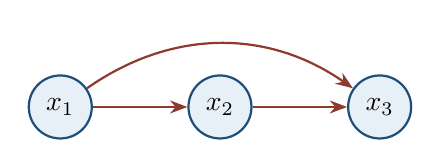
\begin{tikzpicture}[
  node/.style={circle, draw=navy, thick, minimum size=8mm, inner sep=0pt, fill=navysoft},
  arr/.style={-{Stealth[length=2.2mm]}, thick, draw=burgundy}
]
\node[node] (x1) {$x_1$};
\node[node, right=12mm of x1] (x2) {$x_2$};
\node[node, right=12mm of x2] (x3) {$x_3$};
\draw[arr] (x1) -- (x2);
\draw[arr] (x1) to[bend left=35] (x3);
\draw[arr] (x2) -- (x3);
\end{tikzpicture}
\end{center}
\begin{center}
\textcolor{muted}{\small An autoregressive factorization. Each variable is conditioned only on the variables already generated.}
\end{center}

\section{Markov models and mixture transitions}

Context length at position $i$ is $\ell_i=\min(m,i-1)$. A conditional table on $K$ symbols has $K-1$ free entries per context. An inhomogeneous Markov model of order $m$ on length $n$ therefore has
\begin{resultbox}[Inhomogeneous and homogeneous parameter counts]
\[
N_m^{\mathrm{nh}}
=(K^m-1)+(n-m)(K-1)K^m,\qquad
N_m^{\mathrm{h}}=K^{m+1}-1.
\]
\end{resultbox}
The difference is $(n-m-1)(K-1)K^m$, which vanishes when $n=m+1$: then both families equal the full simplex.

A mixture transition kernel $c_{ab}=\lambda t_1(a)+(1-\lambda)t_2(b)$ on binary contexts forces the cross difference $c_{00}-c_{01}-c_{10}+c_{11}=0$. Its image is a full-dimensional subset of a three-dimensional affine subspace of the free conditional table $[0,1]^4$, so five nominal parameters overcount a three-dimensional model.

\section{KL projection onto autoregressive tables}

For $q(x)=\prod_i q_i(x_i\given c_i)$ and $q^\star(x)=\prod_i p(x_i\given c_i)$,
\begin{resultbox}[Closest autoregressive table]
\[
\KL(p\Vert q)=\KL(p\Vert q^\star)+\sum_i\E\bigl[\KL\bigl(p(\cdot\given c_i)\Vert q_i(\cdot\given c_i)\bigr)\bigr].
\]
\end{resultbox}
Each inner KL is nonnegative, so $q^\star$ is the unique closest member of the inhomogeneous family. The gap $\KL(p\Vert q^\star)$ equals a sum of conditional mutual informations between $x_i$ and the discarded distant past given the window. Maximum likelihood on fully observed sequences estimates those conditionals by empirical counts. Homogeneous models replace the position-dependent kernels by a single tied kernel equal to the mixture of the true conditionals weighted by context frequencies.

\section{FVSBN and NADE}

A fully visible sigmoid belief network replaces the table by a logistic regression on the past:
\[
p(x_d=1\given x_{<d})=\sigma\Bigl(b_d+\sum_{k<d}W_{dk}x_k\Bigr).
\]
Step $d$ costs $d$ parameters, and the total is $D(D+1)/2$. The map from parameters to distributions is injective for this linear-logit family, so that count is the dimension of the model. The family is exactly the set of positive pmfs whose autoregressive logits, in the fixed order, are affine. Equality with the full simplex $\dim\mathcal P_D=2^D-1$ holds only for $D=1,2$.

NADE shares one hidden state across the conditionals,
\[
h_d=\phi\Bigl(c+\sum_{k<d}W_{:,k}x_k\Bigr),\qquad
p(x_d=1\given x_{<d})=\sigma(v_d^\top h_d+b_d).
\]
Sharing $W$ makes the parameter count $D_h(2D-1)+D$, linear in $D$ rather than quadratic. The recurrence $a_{d+1}=a_d+W_{:,d}x_d$ evaluates every conditional without recomputing the sum from scratch, cutting the scalar multiplications in $\log p(x)$ from $O(D^2 D_h)$ to $O(D D_h)$. Sampling remains sequential: $a_d$ depends on the previously drawn bits. Likelihood of a fully observed $x$ can still be evaluated in parallel across coordinates.

The Bernoulli negative log-likelihood in the logit $z$ has derivative $\sigma(z)-x$. Backpropagating through NADE accumulates $\partial L/\partial a_d$ into shared parameters by a single reverse suffix sum of cost $O(D D_h)$. With $\phi=\tanh$, sign flips and permutations of hidden units leave $p_\theta$ unchanged, giving a hyperoctahedral fiber of size $D_h!\,2^{D_h}$.

Real NADE uses the same hidden state and emits a Gaussian conditional, with mean linear in $h_d$ and variance $\exp(s_d)$; the Gaussian NLL calculus of Chapter~\ref{ch:gauss} then replaces the Bernoulli score.

\begin{intbox}
Likelihood of a fully observed $x$ can be computed in parallel across coordinates, because every past bit is already known. Sampling cannot. Coordinate $d$ is drawn only after coordinates $1,\ldots,d-1$ exist. Lecture~3 says this in one line, and MAF inherits it.
\end{intbox}

\begin{practbox}[FVSBN versus full simplex]
For $D=3$, compare $\dim\mathcal F_3=D(D+1)/2$ with $\dim\mathcal P_3=2^D-1$. Can an FVSBN represent the parity distribution that puts mass $\theta/4$ on odd strings and $(1-\theta)/4$ on even strings when $\theta\ne 1/2$?
\end{practbox}
\begin{solbox}
$\dim\mathcal F_3=6<7=\dim\mathcal P_3$. For the parity law the last logit has second-order interaction $4\log(\theta/(1-\theta))\ne 0$, which no affine function of $(x_1,x_2)$ can match. So no FVSBN represents that $p$, in any order.
\end{solbox}

\section{MADE masks}

MADE imposes the autoregressive constraint with binary masks so that one forward pass evaluates every conditional. Number the hidden units by the largest input index they may depend on. A hidden unit with index $m$ may read inputs of index at most $m$. An output unit for coordinate $d$ may read hidden units of index strictly less than $d$. The strict inequality at the output stops $x_d$ from depending on itself.

\begin{resultbox}[Mask connectivity]
With degrees $m^0$ on inputs/outputs and $m^1$ on hidden units,
\[
[M^W]_{ki}=\mathbf 1\{m^1(k)\ge m^0(i)\},\qquad
[M^V]_{dk}=\mathbf 1\{m^0(d)>m^1(k)\}.
\]
A dependence of position $j$ on earlier position $r$ has a path if and only if some hidden degree lies in $\{r,\ldots,j-1\}$. One unit of each degree $1,\ldots,D-1$ is necessary and sufficient for full connectivity of the ordering.
\end{resultbox}
The same degree rule between successive hidden layers preserves the invariant at any depth. Weakening the output rule to a non-strict inequality allows $\lambda_d$ to depend on $x_d$, destroying normalization of the product of Bernoulli factors.

\begin{practbox}[A mask you can draw]
For $D=3$ and one hidden layer with indices $(1,2,2)$, say which inputs each output may use.
\end{practbox}
\begin{solbox}
Output $1$ may use hidden units of index $<1$. There are none. So $p(x_1)$ is unconditional. Output $2$ may use the hidden unit of index $1$, which itself may see only $x_1$. Output $3$ may use all three hidden units, hence $x_1$ and $x_2$, and not $x_3$. That is an autoregressive family.
\end{solbox}

\section{Graphs, orderings, and d-separation of parents}

A directed acyclic graph defines a legal joint by multiplying one conditional per node, given its parents. A topological order is an order in which every parent appears before its child. Many orders can be legal. Induct along any topological order: each conditional sums to one in its child, so the product is a pmf. Acyclicity is what supplies the order.

A directed cycle does not define a joint by the same multiplication: the conditionals refer to each other and need not be normalizable. For a two-node cycle the sum of the product of conditionals is $Z=1+(\theta_0-\theta_1)(\varphi_0-\varphi_1)$, equal to one if and only if at least one conditional ignores its parent.

A rooted forest is the special case in which each node has at most one parent. The number of topological orders of a rooted forest on $n$ vertices is $n!/\prod_v h_v$, where $h_v$ is the subtree size at $v$. Restoring an edge keeps exactly those forest orders that also put the new parent before the child. Markov chains are the path case, homogeneous when the conditional does not depend on time, inhomogeneous when it does.

The KL projection of a full joint onto an autoregressive family is the set of conditional tables of the true joint, in that order. The KL gap equals a conditional mutual information: the information about $x_d$ that the discarded non-parents still carry. Maximum likelihood on a fully observed table estimates those conditionals by counts.

\section{Gaussian class-conditional Bayes classifiers}

When class-conditional laws are Gaussian, the Bayes classifier is logistic in the features after taking the logit of $p(y=1\given x)$. Shared covariance cancels the pure quadratic terms and leaves an affine logit $w^\top x+b$ with $w=\Sigma^{-1}(\mu_1-\mu_0)$. Unequal covariances leave a quadratic discriminant. The generative shared-covariance model has $1+2D+D(D+1)/2$ parameters; logistic regression has only $D+1$. The fiber over a fixed $(w,b)$ is diffeomorphic to $\{\Sigma\succ 0\}\times\R^D$.

Masking coordinates and classifying from the marginal of the observed block inverts $\Sigma_{VV}$, not the conditional covariance $S_{V\mid M}$. Mean-imputing the masked block inside the full-data discriminant uses a different coefficient and agrees with the marginal Bayes rule only under an orthogonality condition on the class-mean gap.

The shared-covariance MLE is the class proportion, the two class sample means, and the pooled scatter; uniqueness follows from $\lambda-1-\log\lambda\ge 0$. Logistic NLL is convex, but under linear separation the unpenalized MLE does not exist. An $\ell_2$ penalty on $w$ restores a unique minimizer.

\section{Homework 1 problems}

\begin{hwqbox}[Homework 1, problem 3.1]
Derive the parameter counts $N_m^{\mathrm{nh}}$ and $N_m^{\mathrm{h}}$ for inhomogeneous and homogeneous Markov models of order $m$ on length $n$ over an alphabet of size $K$. Check the cases $m=0$ and $m=n-1$, and interpret the difference.
\end{hwqbox}
\begin{hwsolbox}[Homework 1, problem 3.1]
\[
N_m^{\mathrm{nh}}
=\sum_{i=1}^n(K-1)K^{\min(m,i-1)}
=(K^m-1)+(n-m)(K-1)K^m.
\]
The sum splits into the growing prefix $i\le m$, which contributes $K^m-1$, and the $n-m$ full windows of length $m$. Checks: $m=0$ gives $N=n(K-1)$; $m=n-1$ gives $N=K^n-1$, the full simplex.

For the homogeneous subfamily, the prefix $x_{1:m}$ has an arbitrary pmf ($K^m-1$ parameters) and all later positions share one kernel ($K^m(K-1)$ parameters):
\[
N_m^{\mathrm{h}}=K^m-1+(K-1)K^m=K^{m+1}-1.
\]
Same checks: $m=0$ gives $K-1$; $m=n-1$ gives $K^n-1$. Difference:
\[
N_m^{\mathrm{nh}}-N_m^{\mathrm{h}}=(n-m-1)(K-1)K^m.
\]
If $n=m+1$, the difference is $0$: both families equal the full simplex.
\end{hwsolbox}

\begin{hwqbox}[Homework 1, problem 3.1(a)]
For the binary mixture transition $c_{ab}=\lambda t_1(a)+(1-\lambda)t_2(b)$, show that the image lies in the hyperplane $c_{00}-c_{01}-c_{10}+c_{11}=0$, that every cube point on that hyperplane is attained, and that the model dimension is $3$.
\end{hwqbox}
\begin{hwsolbox}[Homework 1, problem 3.1(a)]
The cross difference vanishes because both $c_{00}-c_{01}$ and $c_{10}-c_{11}$ equal $(1-\lambda)(t_2(0)-t_2(1))$. Conversely, every $c\in[0,1]^4$ on this hyperplane is attained: additivity gives $c_{ab}=A_a+B_b$, and the normalized choice $B_b=\min_a c_{ab}$, $A_a=c_{ab}-B_b$ yields nonnegative $A,B$ with $\max A+\max B\le 1$. Set $\lambda=\max A$ and rescale to obtain $\alpha,\beta\in[0,1]^2$.

The image is a full-dimensional subset of a $3$-dimensional affine subspace, intersected with the cube, with nonempty relative interior. Its dimension is $3$. A free conditional table has dimension $4$. The five nominal parameters therefore overcount: the fiber of a generic table has dimension $5-3=2$. The model cannot represent a conditional with a nonzero interaction, for example $c=(1,0,0,1)$.
\end{hwsolbox}

\begin{hwqbox}[Homework 1, problem 3.2]
Prove that the unique closest member of the inhomogeneous autoregressive family $Q_m^{\mathrm{nh}}$ to a positive joint $p$, in forward KL, is $q^\star(x)=\prod_i p(x_i\given c_i)$.
\end{hwqbox}
\begin{hwsolbox}[Homework 1, problem 3.2]
For $q(x)=\prod_i q_i(x_i\given c_i)$ and $q^\star(x)=\prod_i p(x_i\given c_i)$,
\begin{align*}
\KL(p\Vert q)
&=\KL(p\Vert q^\star)+\sum_{i=1}^n\E_p\Big[\log\frac{p(x_i\given c_i)}{q_i(x_i\given c_i)}\Big]\\
&=\KL(p\Vert q^\star)+\sum_{i=1}^n\E\big[\KL\big(p(\cdot\given c_i)\,\|\,q_i(\cdot\given c_i)\big)\big].
\end{align*}
Each inner KL is nonnegative. Hence $\KL(p\Vert q)\ge\KL(p\Vert q^\star)$, with equality if and only if $q_i(\cdot\given c)=p(\cdot\given c)$ for every $i$ and every context (all contexts have positive probability because $p>0$). The unique closest member is $q^\star$.
\end{hwsolbox}

\begin{hwqbox}[Homework 1, problem 3.2(a)]
Express the gap $\KL(p\Vert q^\star)$ as a sum of conditional mutual informations. Specialize to $m=0$.
\end{hwqbox}
\begin{hwsolbox}[Homework 1, problem 3.2(a)]
Chain rule: $\log p(x)=\sum_i\log p(x_i\given x_{<i})$ and $\log q^\star(x)=\sum_i\log p(x_i\given c_i)$. For $i\le m+1$ the window $c_i$ is the entire past, so those terms cancel. For $i\ge m+2$,
\[
\log\frac{p(x_i\given x_{<i})}{p(x_i\given c_i)}
\]
is the integrand of $I(X_i;X_{1:i-m-1}\given X_{i-m:i-1})$. Therefore
\[
\KL(p\Vert q^\star)=\sum_{i=m+2}^{n}I\big(X_i;\,X_{1:i-m-1}\given X_{i-m:i-1}\big).
\]
It is zero if and only if $p$ itself factors through windows of length $m$. For $m=0$,
\[
\KL(p\Vert q^\star)=\sum_{i=2}^n I(X_i;X_{1:i-1})=\sum_i H(X_i)-H(X),
\]
the total correlation of $p$.
\end{hwsolbox}

\begin{hwqbox}[Homework 1, problem 3.2(b)]
Show that maximum likelihood tables for an inhomogeneous Markov model are the empirical conditionals, and relate this to the KL projection of problem~3.2.
\end{hwqbox}
\begin{hwsolbox}[Homework 1, problem 3.2(b)]
The average log-likelihood of $N$ i.i.d.\ sequences is $\sum_i\sum_{c,k}\hat p_i(c,k)\log q_i(k\given c)$. For each $(i,c)$ with a positive count, the Lagrangian of $\sum_k N_i(c,k)\log q_k$ subject to $\sum_k q_k=1$ has solution
\[
\hat q_i(k\given c)=\frac{N_i(c,k)}{N_i(c)}.
\]
These are the conditionals of the empirical distribution $\hat p$. Maximizing the likelihood is the same as minimizing $\KL(\hat p\Vert q)$, whose unique minimizer on tables that are seen in the data is the $q^\star$ of problem~3.2 built from $\hat p$. Unseen contexts are unidentified.
\end{hwsolbox}

\begin{hwqbox}[Homework 1, problem 3.2(c)]
Derive the best homogeneous model $q_h^\star$ and express the excess KL relative to the inhomogeneous projection as a weighted sum of KLs between position-dependent kernels and the tied kernel.
\end{hwqbox}
\begin{hwsolbox}[Homework 1, problem 3.2(c)]
$\log q=\log\pi(x_{1:m})+\sum_{i>m}\log T(x_i\given c_i)$. The prefix expectation $\E\log\pi(X_{1:m})$ is maximized uniquely by the true marginal $\pi^\star=p_{1:m}$. The shared kernel maximizes
\[
\sum_{i=m+1}^n\sum_{c,k}p_i(c,k)\log T(k\given c),
\]
so
\[
T^\star(k\given c)=\frac{\sum_{i>m}p_i(c,k)}{\sum_{i>m}p_i(c)}
=\sum_{i=m+1}^n w_i(c)\,p_i(k\given c),
\]
with weights $w_i(c)=p_i(c)/\sum_{j>m}p_j(c)$. The excess KL is
\[
\KL(p\Vert q_h^\star)-\KL(p\Vert q^\star)
=\sum_{i=m+1}^n\sum_c p_i(c)\,\KL\big(p_i(\cdot\given c)\,\Vert\,T^\star(\cdot\given c)\big).
\]
It vanishes if and only if $p_i(\cdot\given c)$ does not depend on $i$, for every context that occurs after time $m$.
\end{hwsolbox}

\begin{hwqbox}[Homework 1, problem 3.3]
For the DAG of Figure~1 (edges $B\to E$, $B\to G$, $E\to G$, $A\to D$, $A\to C$, $D\to F$, $C\to F$), write the factorization, count binary CPT parameters, and prove that any finite DAG factorization is normalized.
\end{hwqbox}
\begin{hwsolbox}[Homework 1, problem 3.3]
Parents: $A,B$ are roots; $\mathrm{pa}(C)=\{A\}$, $\mathrm{pa}(D)=\{A\}$, $\mathrm{pa}(E)=\{B\}$, $\mathrm{pa}(F)=\{C,D\}$, $\mathrm{pa}(G)=\{B,E\}$.
\[
p(x)=p(x_A)p(x_B)p(x_C\given x_A)p(x_D\given x_A)p(x_E\given x_B)p(x_F\given x_C,x_D)p(x_G\given x_B,x_E).
\]
Binary conditional probability tables contribute $2^{|\mathrm{pa}(v)|}$ free parameters: $1+1+2+2+2+4+4=16$.

\textbf{Normalization on any finite DAG.} Induct along a topological order $v_1,\ldots,v_n$. The empty product sums to $1$. Given that the marginal of the first $t-1$ variables is a pmf,
\[
\sum_{x_{v_t}}p(x_{v_t}\given x_{\mathrm{pa}(v_t)})=1
\]
for every parent configuration, and the parents are among the previous variables. Multiplying and summing over $x_{v_t}$ leaves the previous marginal. After $n$ steps the product sums to $1$. Acyclicity is what supplies the topological order.
\end{hwsolbox}

\begin{hwqbox}[Homework 1, problem 3.3(a)]
Count the valid topological orderings of Figure~1, and give the probability that a uniform random permutation is valid.
\end{hwqbox}
\begin{hwsolbox}[Homework 1, problem 3.3(a)]
On $\{B,E,G\}$ the only order is $B,E,G$. On $\{A,C,D,F\}$, $A$ is first, $F$ is last, and $\{C,D\}$ is free: $2$ orders. Interleaving a block of $3$ with a block of $4$ can be done in $\binom{7}{3}$ ways. Total:
\[
\binom{7}{3}\cdot 1\cdot 2=70.
\]
Out of $7!=5040$ permutations, the probability is $70/5040=1/72$.
\end{hwsolbox}

\begin{hwqbox}[Homework 1, problem 3.3(b)]
Delete $C\to F$ and $E\to G$ to obtain a rooted forest. Count topological orders by the subtree-size formula, then restore each edge (and both) by conditioning on the forest orders, and compare with problem~3.3(a).
\end{hwqbox}
\begin{hwsolbox}[Homework 1, problem 3.3(b)]
For a rooted tree in which every node has at most one parent and edges point away from the root, the number of orders in which every node precedes its descendants is $n!/\prod_v h_v$, where $h_v$ is the subtree size at $v$. A forest extends by the same formula.

Delete $C\to F$ and $E\to G$. The forest is $B$ with leaf children $E,G$ ($h_B=3$, $h_E=h_G=1$) and $A$ with child $C$ and child $D\to F$ ($h_A=4$, $h_D=2$, $h_C=h_F=1$). Then $\prod_v h_v=4\cdot 3\cdot 2=24$ and $7!/24=210$.

Restoring $E\to G$: $E$ and $G$ are symmetric leaves, so exactly half survive: count $105$. Restoring $C\to F$: inside $A$'s tree the three equally likely orders of $\{C,D,F\}$ with $D$ before $F$ are $CDF$, $DCF$, $DFC$, and the first two have $C$ before $F$. Fraction $2/3$, count $140$. Restoring both: fraction $\tfrac12\cdot\tfrac23=\tfrac13$, count $70$, matching problem~3.3(a).
\end{hwsolbox}

\begin{hwqbox}[Homework 1, problem 3.3(c)]
For a two-node directed cycle with binary conditionals parameterized by $(\theta_0,\theta_1)$ and $(\varphi_0,\varphi_1)$, compute the normalizing constant $Z$ of the product of conditionals, characterize when $Z=1$, and explain why dropping $\log Z$ from maximum likelihood is incorrect when $Z$ depends on the parameters.
\end{hwqbox}
\begin{hwsolbox}[Homework 1, problem 3.3(c)]
\begin{align*}
q(0,0)&=(1-\theta_0)(1-\varphi_0),&
q(1,0)&=\theta_0(1-\varphi_1),\\
q(0,1)&=(1-\theta_1)\varphi_0,&
q(1,1)&=\theta_1\varphi_1.
\end{align*}
Summing and cancelling leaves $Z=1+(\theta_0-\theta_1)(\varphi_0-\varphi_1)$. So $Z=1$ if and only if $\theta_0=\theta_1$ or $\varphi_0=\varphi_1$, i.e.\ at least one of the two conditionals ignores its parent. Otherwise the product is not a pmf.

Maximum likelihood needs $\sum_x\log(q_\theta(x)/Z(\theta))$. Dropping $\log Z(\theta)$ is not the log-likelihood as soon as $Z$ depends on $\theta$: the score misses $-\nabla\log Z$, and the parameters remain coupled through the normalizer, which a DAG factorization would have avoided.
\end{hwsolbox}

\begin{hwqbox}[Homework 1, problem 4.1]
Count parameters of FVSBN and NADE on $\{0,1\}^D$. For $D=784$, find the largest hidden width $D_h$ for which NADE has fewer parameters than FVSBN.
\end{hwqbox}
\begin{hwsolbox}[Homework 1, problem 4.1]
FVSBN: one bias per coordinate, and $w_d\in\R^{d-1}$ for $d\ge 2$.
\[
D+\sum_{d=2}^D(d-1)=D+\frac{D(D-1)}{2}=\frac{D(D+1)}{2}.
\]
NADE: $W$ has $D_h(D-1)$ entries, $c$ has $D_h$, each of the $D-1$ conditionals $d\ge 2$ has a vector $v_d$ and a bias, and $b_1$ is one more bias.
\[
D_h(D-1)+D_h+(D-1)D_h+D=D_h(2D-1)+D.
\]
NADE is smaller when $D_h<D(D-1)/(2(2D-1))$. For $D=784$, the threshold is $306936/1567\approx 195.875$. The largest such integer is $D_h=195$.
\end{hwsolbox}

\begin{hwqbox}[Homework 1, problem 4.1(a)]
Count scalar multiplications inside the affine maps of $\log p(x)$ for FVSBN, for NADE recomputing each $a_d$, and for NADE with the recursion $a_{d+1}=a_d+W_{:,d}x_d$. Evaluate at $D=784$, $D_h=500$.
\end{hwqbox}
\begin{hwsolbox}[Homework 1, problem 4.1(a)]
Count products inside the affine maps, not evaluations of $\sigma$, $\log$, or $\phi$.
\begin{itemize}
\item FVSBN: $w_d^\top x_{<d}$ costs $d-1$ products. Total $D(D-1)/2$. At $D=784$: $306936$.
\item NADE, recomputing each $a_d$: total $D_h(D-1)(D+2)/2$. At $D=784$, $D_h=500$: $153859500$.
\item NADE, recursion: total $2(D-1)D_h$. At the same size: $783000$.
\end{itemize}
\end{hwsolbox}

\begin{hwqbox}[Homework 1, problem 4.1(b)]
Explain why sampling from NADE stays sequential, while evaluating $\log p(x)$ for a fixed $x$ can be parallelized across coordinates.
\end{hwqbox}
\begin{hwsolbox}[Homework 1, problem 4.1(b)]
To sample $x_d$ one needs the conditional, whose input $a_d$ depends on $x_1,\ldots,x_{d-1}$. Those bits are not known until the previous draws have been made, so the $D$ draws form a chain. The recursion removes repeated work; it does not remove that chain.

For a fixed $x$, every bit is already known. Each $a_d=\sum_{k<d}W_{:,k}x_k$ is a function of known numbers, and the $D$ conditionals may be evaluated independently, in parallel.
\end{hwsolbox}

\begin{hwqbox}[Homework 1, problem 4.2]
Derive the NADE gradients of the Bernoulli NLL with respect to $z_d$, $b_d$, $v_d$, $h_d$, $a_d$, $c$, and the columns of $W$.
\end{hwqbox}
\begin{hwsolbox}[Homework 1, problem 4.2]
The Bernoulli negative log-likelihood in the logit $z$ has derivative $\sigma(z)-x$. With $\delta_d=\sigma(z_d)-x_d$,
\[
\frac{\partial L}{\partial z_d}=\delta_d.
\]
Consequences, using $z_1=b_1$ and $z_d=v_d^\top h_d+b_d$ for $d\ge 2$:
\begin{align*}
\frac{\partial L}{\partial b_d}&=\delta_d &&(1\le d\le D),\\
\frac{\partial L}{\partial v_d}&=\delta_d h_d &&(d\ge 2),\\
\frac{\partial L}{\partial h_d}&=\delta_d v_d &&(d\ge 2),\\
\frac{\partial L}{\partial a_d}&=\phi'(a_d)\odot(\delta_d v_d) &&(d\ge 2).
\end{align*}
The shared parameters touch every later conditional:
\[
\frac{\partial L}{\partial c}=\sum_{d=2}^D\frac{\partial L}{\partial a_d},\qquad
\frac{\partial L}{\partial W_{:,k}}=x_k\sum_{d=k+1}^D\frac{\partial L}{\partial a_d}.
\]
\end{hwsolbox}

\begin{hwqbox}[Homework 1, problem 4.2(a)]
Describe the $O(DD_h)$ backward accumulation for $\partial L/\partial W$, the MAP objective under a Gaussian prior (weight decay), and the $\tanh$ sign-and-permutation symmetries with their order $D_h!\,2^{D_h}$.
\end{hwqbox}
\begin{hwsolbox}[Homework 1, problem 4.2(a)]
Write $g_d=\partial L/\partial a_d$. After one forward pass set $S_{D-1}=g_D$ and $S_k=g_{k+1}+S_{k+1}$ while $k$ runs from $D-2$ down to $1$. Then $\partial L/\partial W_{:,k}=x_k S_k$. The accumulation is another $O(DD_h)$ pass.

With $N$ observations and prior $\theta\sim\N(0,\tau^2 I)$, the negative log posterior, up to an additive constant, is
\[
J(\theta)=\sum_{n=1}^N L(x^{(n)};\theta)+\frac{1}{2\tau^2}\Vert\theta\Vert^2.
\]
Its gradient is the sum of the data gradients plus $\theta/\tau^2$ (weight decay with coefficient $1/\tau^2$).

Symmetries of $\phi=\tanh$: for each hidden unit $j$ and each sign $\varepsilon_j\in\{\pm 1\}$, flip the signs of $c_j$, $W_{j,:}$, and every $(v_d)_j$. Then every logit is unchanged. Together with permutations of hidden units this is the hyperoctahedral action of order $D_h!\,2^{D_h}$. For a generic $\theta$ that order is a lower bound on the size of the fiber. There is no continuous scale symmetry for $\tanh$.
\end{hwsolbox}

\begin{hwqbox}[Homework 1, problem 4.3]
Characterize the FVSBN family $\mathcal F_D$, prove injectivity of the parameter map, compute $\dim\mathcal F_D$, and determine for which $D$ one has $\mathcal F_D=\mathcal P_D$.
\end{hwqbox}
\begin{hwsolbox}[Homework 1, problem 4.3]
For a positive pmf the logits $\ell_d(x_{<d})=\log\frac{p(x_d=1\given x_{<d})}{p(x_d=0\given x_{<d})}$ may be arbitrary real functions of the past. An FVSBN forces each logit to be affine, so $\mathcal F_D$ is exactly the set of positive pmfs whose autoregressive logits, in the fixed order, are affine.

The map from parameters to pmfs is injective: an affine function on the cube determines its coefficients by $b=\ell(0)$ and $w_i=\ell(e_i)-\ell(0)$. The parameter count is $D(D+1)/2$, and the parameter domain $\R^{D(D+1)/2}$ is mapped diffeomorphically onto $\mathcal F_D$ by the coordinatewise sigmoid. Hence $\dim\mathcal F_D=D(D+1)/2$.

$\dim\mathcal P_D=2^D-1$. Equality holds for $D=1$ and $D=2$. For $D=3$, $6<7$, and $2^D-1$ grows faster afterwards. Only $D=1,2$.
\end{hwsolbox}

\begin{hwqbox}[Homework 1, problem 4.3(a)]
Show that the parity distribution with mass $\theta/4$ on odd strings and $(1-\theta)/4$ on even strings ($\theta=1/10$) is not an FVSBN, in any order.
\end{hwqbox}
\begin{hwsolbox}[Homework 1, problem 4.3(a)]
There are four odd strings and four even strings, and the masses sum to $1$. By symmetry it is enough to rule out the order $(x_1,x_2,x_3)$. The marginal of $(x_1,x_2)$ is uniform on four points. The conditional $p(x_3=1\given x_1,x_2)$ equals $\theta$ when $x_1\oplus x_2=0$ and equals $1-\theta$ when $x_1\oplus x_2=1$. With $L=\log(\theta/(1-\theta))=\log(1/9)$,
\[
\ell(0,0)=\ell(1,1)=L,\qquad \ell(1,0)=\ell(0,1)=-L.
\]
An affine function would satisfy $\ell(1,1)-\ell(1,0)-\ell(0,1)+\ell(0,0)=0$. The actual second-order interaction is $4L=-4\log 9\ne 0$. No FVSBN represents $p$, in any order.
\end{hwsolbox}

\begin{hwqbox}[Homework 1, problem 4.3(b)]
Construct a ReLU NADE of width $D-1$ that represents the parity distribution for general $D$.
\end{hwqbox}
\begin{hwsolbox}[Homework 1, problem 4.3(b)]
Let $L=\log(\theta/(1-\theta))$ and $D_h=D-1$. Set $b_1=0$, and $v_d=0$, $b_d=0$ for $2\le d\le D-1$. Then the first $D-1$ bits are i.i.d.\ uniform.

For the last conditional, let $s=\sum_{k=1}^{D-1}x_k$ and use one hidden unit per threshold: $c_j=1-j$, $W=\mathbf 1_{D_h\times(D-1)}$. Then $h_j=\mathrm{ReLU}(s-(j-1))$, and on integers $s$ one has $\mathbf 1_{s\ge k}=h_k-h_{k+1}$ (with $h_D:=0$). Taking $g(s)=L(-1)^s$ and collecting coefficients of the $h_j$ gives
\[
b_D=L,\qquad v_{D,1}=-2L,\qquad v_{D,j}=4L(-1)^j\ \text{for }j=2,\ldots,D-1.
\]
Then $z_D=L$ on even popcount and $z_D=-L$ on odd popcount, so the conditional probability that the total parity is odd equals $\theta$.
\end{hwsolbox}

\begin{hwqbox}[Homework 1, problem 4.4]
For Figure~2 with degrees $m^0(x)=(2,4,1,3)$ and the listed hidden degrees, write the masks $M^W$ and $M^V$, count the ones, list the variables each $\lambda_d$ can depend on in the order $x_3,x_1,x_4,x_2$, and find the smallest width that drops no dependence the order allows.
\end{hwqbox}
\begin{hwsolbox}[Homework 1, problem 4.4]
\[
[M^W]_{ki}=\mathbf 1\{m^1(k)\ge m^0(i)\},\qquad
[M^V]_{dk}=\mathbf 1\{m^0(d)>m^1(k)\}.
\]
Columns of $M^W$ are $(x_1,x_2,x_3,x_4)$ with degrees $(2,4,1,3)$. Rows are $h_1,\ldots,h_6$:
\[
M^W=\begin{pmatrix}
0&0&1&0\\
1&0&1&1\\
1&0&1&1\\
0&0&1&0\\
1&0&1&1\\
0&0&1&0
\end{pmatrix},\qquad
\#\{1\}=12.
\]
Rows of $M^V$ are $\lambda_1,\ldots,\lambda_4$:
\[
M^V=\begin{pmatrix}
1&0&0&1&0&1\\
1&1&1&1&1&1\\
0&0&0&0&0&0\\
1&0&0&1&0&1
\end{pmatrix},\qquad
\#\{1\}=12.
\]
In the order $x_3,x_1,x_4,x_2$: $\lambda_3$ sees none; $\lambda_1$ sees $x_3$; $\lambda_4$ sees $x_3$ only (not $x_1$); $\lambda_2$ sees $x_3,x_1,x_4$. The network is not as expressive as a general autoregressive model for this order: the missing dependence is $x_1\to\lambda_4$.

Smallest width that drops nothing the order allows: the consecutive pair $r\to r+1$ forces a hidden unit of degree exactly $r$, so $H\ge D-1$, and one unit of each degree $1,\ldots,D-1$ is sufficient.
\end{hwsolbox}

\begin{hwqbox}[Homework 1, problem 4.4(a)]
Show that the same degree rule at every hidden layer preserves autoregressive normalization at any depth, and that a non-strict output mask can break normalization.
\end{hwqbox}
\begin{hwsolbox}[Homework 1, problem 4.4(a)]
Use the same rule between successive hidden layers: a unit may read a previous unit only when its own degree is at least the previous unit's degree. By induction on depth, a unit of degree $m$ depends only on inputs of degree at most $m$. The output $\lambda_d$ reads only units of degree $<m^0(d)$, hence only inputs of degree $<m^0(d)$. It does not depend on $x_d$ or on any later variable. Therefore each factor $\mathrm{Bernoulli}(x_d\given\lambda_d)$ is a conditional probability given the earlier variables in the degree order, and the product is a pmf.

If the output rule is weakened to $\mathbf 1\{m^0(d)\ge m^1(k)\}$, a unit of degree $m^0(d)$ may connect to $\lambda_d$, and that unit may depend on $x_d$ itself. Then $\lambda_d$ depends on $x_d$, the factor is not a conditional distribution in the remaining variables, and $\sum_{x_d}\mathrm{Bernoulli}(x_d\given\lambda_d(x_d))$ need not be $1$.
\end{hwsolbox}

\begin{hwqbox}[Homework 1, problem 4.4(b)]
With hidden degrees i.i.d.\ uniform on $\{1,\ldots,D-1\}$, compute $\E[\#\{M^W=1\}]$ and $\E[\#\{M^V=1\}]$, the connection probability of an allowed dependence $r\to j$, the probability that all allowed dependences are connected, and $\E[T]$ for the coupon-collector waiting time until every dependence is connected. Evaluate $\E[T]$ at $D=784$.
\end{hwqbox}
\begin{hwsolbox}[Homework 1, problem 4.4(b)]
For an input of degree $r$, $\mathbb P(m^1\ge r)=(D-r)/(D-1)$. Summing over $r$ gives $D/2$. With $H$ independent rows, $\E[\#\{M^W=1\}]=HD/2$. The same sum for outputs gives $\E[\#\{M^V=1\}]=HD/2$.

An allowed dependence $r\to j$, with $j>r$, is connected when at least one hidden degree falls in an interval of $j-r$ integers:
\[
\mathbb P(\text{connected})=1-\Big(1-\frac{j-r}{D-1}\Big)^H.
\]
All allowed dependences are connected simultaneously if and only if every degree in $\{1,\ldots,D-1\}$ appears at least once. By inclusion-exclusion, for $H\ge D-1$,
\[
\mathbb P(\text{all connected})
=\sum_{i=0}^{D-1}(-1)^{D-1-i}\binom{D-1}{i}\Big(\frac{i}{D-1}\Big)^H,
\]
and the probability is $0$ for $H<D-1$. The expected number of hidden units needed until every dependence is connected is
\[
\E[T]=(D-1)\sum_{k=1}^{D-1}\frac1k.
\]
For $D=784$, $M=783$ and $\E[T]=783\,H_{783}\approx 5669.69$.
\end{hwsolbox}

\begin{hwqbox}[Homework 1, problem 6.1]
Derive the Bayes classifier $p(y=1\given x)=\sigma(a(x))$ for class-conditional Gaussians, specialize to shared covariance (affine logit) and unequal covariances (quadratic discriminant).
\end{hwqbox}
\begin{hwsolbox}[Homework 1, problem 6.1]
\[
p(y=1\given x)=\sigma(a(x)),\qquad
a(x)=\log\frac{\pi}{1-\pi}+\log\N(x\given\mu_1,\Sigma_1)-\log\N(x\given\mu_0,\Sigma_0).
\]
Expanding the quadratic forms,
\begin{align*}
a(x)&=\log\frac{\pi}{1-\pi}-\tfrac12\log\frac{\det\Sigma_1}{\det\Sigma_0}\\
&\quad+\tfrac12(x-\mu_0)^\top\Sigma_0^{-1}(x-\mu_0)-\tfrac12(x-\mu_1)^\top\Sigma_1^{-1}(x-\mu_1).
\end{align*}
Shared covariance $\Sigma_0=\Sigma_1=\Sigma$: the pure quadratic terms cancel and
\[
a(x)=w^\top x+b,\qquad
w=\Sigma^{-1}\Delta,\qquad
b=-w^\top\bar\mu+\log\frac{\pi}{1-\pi},
\]
with $\Delta=\mu_1-\mu_0$ and $\bar\mu=\tfrac12(\mu_0+\mu_1)$. Unequal covariances leave
\[
a(x)=x^\top Q x+L^\top x+c
\]
with $Q=\tfrac12(\Sigma_0^{-1}-\Sigma_1^{-1})$, $L=\Sigma_1^{-1}\mu_1-\Sigma_0^{-1}\mu_0$, and the corresponding constant $c$. This is the quadratic discriminant.
\end{hwsolbox}

\begin{hwqbox}[Homework 1, problem 6.1(a)]
Count parameters of the shared-covariance generative model and of logistic regression. Describe the fiber over a fixed $(w,b)$ and show that every logistic parameter is realized.
\end{hwqbox}
\begin{hwsolbox}[Homework 1, problem 6.1(a)]
Shared-covariance generative model: $1+2D+D(D+1)/2$ parameters. Logistic regression: $D+1$ parameters. Fix $(w,b)$. Choose $\Sigma\succ 0$ freely and $\bar\mu\in\R^D$ freely. Then $\Delta=\Sigma w$ is determined, the two means are $\bar\mu\pm\Delta/2$, and $\log(\pi/(1-\pi))=b+w^\top\bar\mu$ determines $\pi$. The fiber is diffeomorphic to $\{\Sigma\succ 0\}\times\R^D$ and has dimension $D(D+3)/2$, equal to the difference of the two parameter counts, so the map onto $(w,b)$ is a submersion.
\end{hwsolbox}

\begin{hwqbox}[Homework 1, problem 6.2]
For shared-covariance class-conditional Gaussians, derive the Bayes classifier based only on the observed coordinates $x_V$, and explain why it inverts $\Sigma_{VV}$ rather than $S_{V\mid M}$.
\end{hwqbox}
\begin{hwsolbox}[Homework 1, problem 6.2]
The marginal of a shared-covariance Gaussian is Gaussian with the corresponding block: $x_V\given y=c\sim\N(\mu_{c,V},\Sigma_{VV})$. Part~6.1 in the coordinates $V$ gives
\[
p(y=1\given x_V)=\sigma(w_V^\top x_V+b_V),
\]
\[
w_V=\Sigma_{VV}^{-1}\Delta_V,\qquad
b_V=-\Delta_V^\top\Sigma_{VV}^{-1}\bar\mu_V+\log\frac{\pi}{1-\pi}.
\]
The matrix $S_{V\mid M}$ is the conditional covariance of $x_V$ given $x_M$. It is not the covariance of this marginal. The Bayes rule for the masked problem inverts $\Sigma_{VV}$, not $S_{V\mid M}$.
\end{hwsolbox}

\begin{hwqbox}[Homework 1, problem 6.2(a)]
Show that mean-imputing $x_M\leftarrow\bar\mu_M$ inside the full-data discriminant produces a different coefficient $w_V^{\mathrm{plug}}$, and give sufficient conditions for agreement with the marginal Bayes rule.
\end{hwqbox}
\begin{hwsolbox}[Homework 1, problem 6.2(a)]
The full-data classifier has $w=\Sigma^{-1}\Delta$. Substituting $x_M\leftarrow\bar\mu_M$ produces the logit $w_V^{\mathrm{plug}}\cdot(x_V-\bar\mu_V)+\logit(\pi)$ with
\[
w_V^{\mathrm{plug}}=S_{V\mid M}^{-1}\bigl(\Delta_V-\Sigma_{VM}\Sigma_{MM}^{-1}\Delta_M\bigr),
\]
using the block formula $(\Sigma^{-1})_{VV}=S_{V\mid M}^{-1}$. The Bayes coefficient is $w_V^{\mathrm{Bayes}}=\Sigma_{VV}^{-1}\Delta_V$. Their difference rearranges to the condition
\[
\Sigma_{VM}\Sigma_{MM}^{-1}\bigl(\Delta_M-\Sigma_{MV}\Sigma_{VV}^{-1}\Delta_V\bigr)=0
\]
for agreement for every $x_V$. Sufficient conditions: $\Sigma_{VM}=0$, or $\Delta_M=\Sigma_{MV}\Sigma_{VV}^{-1}\Delta_V$. Mean imputation pretends the masked coordinates were observed and therefore uses the smaller conditional covariance rather than the marginal covariance.
\end{hwsolbox}

\begin{hwqbox}[Homework 1, problem 6.3]
Derive the shared-covariance Gaussian MLE $(\hat\pi,\hat\mu_0,\hat\mu_1,\hat\Sigma)$ and prove uniqueness when $\hat\Sigma\succ 0$ and both classes are nonempty.
\end{hwqbox}
\begin{hwsolbox}[Homework 1, problem 6.3]
The complete log-likelihood separates into a Bernoulli part in $\pi$ and a Gaussian part. $\hat\pi=N_1/N$. For fixed $\Sigma$, the quadratic is minimized in $\mu_c$ at the class sample mean $\hat\mu_c=N_c^{-1}\sum_{y_n=c}x_n$. With pooled scatter $\hat\Sigma=N^{-1}(S_0+S_1)\succ 0$, the profile objective is
\[
L(\Sigma)=-\frac N2\log\det\Sigma-\frac N2\tr(\Sigma^{-1}\hat\Sigma).
\]
If $\lambda_i>0$ are the eigenvalues of $\Sigma^{-1/2}\hat\Sigma\Sigma^{-1/2}$, then
\[
L(\hat\Sigma)-L(\Sigma)=\frac N2\sum_{i=1}^D(\lambda_i-1-\log\lambda_i).
\]
The scalar $\lambda-1-\log\lambda$ is minimized uniquely at $\lambda=1$, so $L(\hat\Sigma)\ge L(\Sigma)$ with equality if and only if $\Sigma=\hat\Sigma$. The MLE is unique.
\end{hwsolbox}

\begin{hwqbox}[Homework 1, problem 6.3(a)]
Write the logistic NLL, prove convexity, and show that under strict linear separation there is no minimizer. Contrast with the generative MLE of problem~6.3.
\end{hwqbox}
\begin{hwsolbox}[Homework 1, problem 6.3(a)]
With $z_n=w^\top x_n+b$ and $\varphi_n=(x_n,1)$,
\[
L(w,b)=\sum_{n=1}^N\big(\log(1+e^{z_n})-y_n z_n\big).
\]
The gradient is $\sum_n(\sigma(z_n)-y_n)\varphi_n$, and
\[
\nabla^2 L=\sum_n\sigma(z_n)(1-\sigma(z_n))\,\varphi_n\varphi_n^\top\succeq 0.
\]
The negative log-likelihood is convex.

Suppose some $(w_0,b_0)$ strictly separates the sample. Along $\theta_t=t(w_0,b_0)$, $t\to\infty$, every class-$1$ logit tends to $+\infty$ and every class-$0$ logit tends to $-\infty$. Each summand tends to $0$, so $L(\theta_t)\to 0$. But for every finite $(w,b)$, every summand is strictly positive, so $L>0$. The infimum $0$ is not attained. There is no minimizer.

By contrast, the generative MLE of problem~6.3 exists and is unique as soon as $\hat\Sigma\succ 0$ and both classes are nonempty, whether or not the sample is linearly separable.
\end{hwsolbox}

\begin{hwqbox}[Homework 1, problem 6.3(b)]
Add $\tfrac\lambda2\lVert w\rVert^2$ with $\lambda>0$, leaving $b$ unpenalized. Prove that the penalized objective is strictly convex and coercive when both classes are nonempty, hence has a unique minimizer even under separation.
\end{hwqbox}
\begin{hwsolbox}[Homework 1, problem 6.3(b)]
The Hessian becomes
\[
\sum_n\sigma_n(1-\sigma_n)\varphi_n\varphi_n^\top+\lambda\,\diag(I_D,0).
\]
For a nonzero direction $(v,c)$: if $v\ne 0$, the penalty contributes $\lambda\lVert v\rVert^2>0$; if $v=0$ and $c\ne 0$, the quadratic form is $c^2\sum_n\sigma_n(1-\sigma_n)>0$. The Hessian is positive definite everywhere, so the penalized objective is strictly convex and has at most one minimizer.

It is coercive when both classes are nonempty. The unpenalized $L$ is nonnegative, so the objective is at least $\tfrac\lambda2\lVert w\rVert^2$ and tends to infinity as $\lVert w\rVert\to\infty$. If $w$ stays bounded and $b\to+\infty$, every class-$0$ term $\log(1+e^{z_n})\to\infty$. If $b\to-\infty$, every class-$1$ term tends to infinity. Thus a minimizer exists, and by strict convexity it is unique. The penalty stops $\lVert w\rVert$ from running off to infinity under separation.
\end{hwsolbox}

\chapter{Variational autoencoders}
\label{ch:vae}

\section{The model}

A latent-variable model says that each observation $x$ was produced by a hidden $z$:
\[
p_\theta(x,z)=p_\theta(x\given z)\,p_\theta(z),\qquad
p_\theta(x)=\int p_\theta(x\given z)\,p_\theta(z)\,dz.
\]
Generation draws $z$ from the prior and then $x$ from the decoder. The integral is the obstacle. It is the marginal likelihood.

\begin{center}
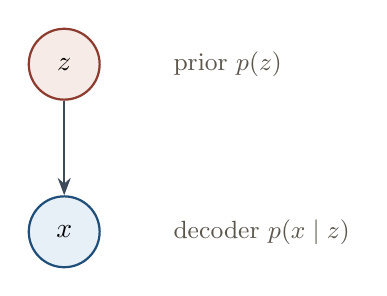
\begin{tikzpicture}[
  lat/.style={circle, draw=burgundy, thick, minimum size=9mm, fill=burgundysoft},
  obs/.style={circle, draw=navy, thick, minimum size=9mm, fill=navysoft},
  arr/.style={-{Stealth[length=2.2mm]}, thick, draw=slate}
]
\node[lat] (z) {$z$};
\node[obs, below=12mm of z] (x) {$x$};
\draw[arr] (z) -- (x);
\node[right=8mm of z, text=muted] {\small prior $p(z)$};
\node[right=8mm of x, text=muted] {\small decoder $p(x\given z)$};
\end{tikzpicture}
\end{center}

For a conditional model the sheet adds a variable $u$, for example a digit label:
\[
p_\theta(x,z\given u)=p_\theta(x\given z,u)\,p_\theta(z\given u).
\]
Every derivation below is the unconditional one with $u$ written next to $x$. The pictures gain arrows from $u$ into the prior and into the decoder.

\section{Two derivations of the ELBO}

Fix a density $q(z)$ that does not depend on $\theta$, positive wherever the posterior is. The marginal is an expectation under $q$:
\[
p_\theta(x)=\E_{z\sim q}\Bigl[\frac{p_\theta(x,z)}{q(z)}\Bigr].
\]
Apply $\log$ and Jensen. The logarithm is concave, so
\begin{equation}
\label{eq:elboj}
\log p_\theta(x)
\ge
\E_{z\sim q}\Bigl[\log\frac{p_\theta(x,z)}{q(z)}\Bigr]
=:\mathcal L(x;\theta,q).
\end{equation}
The right-hand side is the evidence lower bound.

The second derivation starts from the KL between $q$ and the true posterior $p_\theta(z\given x)=p_\theta(x,z)/p_\theta(x)$:
\begin{align*}
\KL(q(z)\Vert p_\theta(z\given x))
&=\E_q\bigl[\log q(z)-\log p_\theta(x,z)+\log p_\theta(x)\bigr]\\
&=\log p_\theta(x)-\E_q\Bigl[\log\frac{p_\theta(x,z)}{q(z)}\Bigr].
\end{align*}
Rearrangement is the identity on Lecture~4, slides~38--39,
\begin{equation}
\label{eq:elbokl}
\log p_\theta(x)=\mathcal L(x;\theta,q)+\KL\bigl(q(z)\Vert p_\theta(z\given x)\bigr).
\end{equation}
Nonnegativity of KL gives $\mathcal L\le\log p_\theta(x)$. The gap is zero if and only if $q(z)=p_\theta(z\given x)$ almost everywhere.

\begin{intbox}
Jensen moves the log inside and produces a bound. The KL identity explains the gap. When you write Homework~2, problem~1.1, do both, and insert $u$ into $p(x,z\given u)$ and $q(z\given x,u)$. Equality is the sentence ``KL is zero only when the densities agree.''
\end{intbox}

\section{Reconstruction minus KL}

Expand $p(x,z)=p(x\given z)p(z)$ inside the ELBO:
\begin{align*}
\mathcal L
&=\E_q[\log p_\theta(x\given z)+\log p_\theta(z)-\log q(z)]\\
&=\E_q[\log p_\theta(x\given z)]-\KL\bigl(q(z)\Vert p_\theta(z)\bigr).
\end{align*}
The first term rewards a decoder that regenerates $x$ from the latent the encoder proposed. The second term penalizes an encoder that wanders away from the prior. For the conditional model,
\begin{equation}
\label{eq:rec}
\mathcal L(\theta,\phi;x,u)
=\E_{q_\phi(z\given x,u)}[\log p_\theta(x\given z,u)]
-\KL\bigl(q_\phi(z\given x,u)\Vert p_\theta(z\given u)\bigr).
\end{equation}

\begin{pitbox}[Posterior collapse]
Suppose $q(z\given x,u)=p(z\given u)$. The KL term in~\eqref{eq:rec} is zero. The gap that remains is
\[
\log p(x\given u)-\mathcal L
=\log\E_{p(z\given u)}[p(x\given z,u)]
-\E_{p(z\given u)}[\log p(x\given z,u)].
\]
That is Jensen's gap for the random variable $p(x\given z,u)$ as $z$ varies. It is strictly positive unless $p(x\given z,u)$ does not depend on $z$.

If the decoder ignores $z$, so that $p(x\given z,u)=p(x\given u)$, Bayes' rule gives $p(z\given x,u)=p(z\given u)$. Matching the encoder to the prior then makes both the KL and the gap vanish. The latent carries no information about $x$. That is posterior collapse. The bound is tight and useless.
\end{pitbox}

\section{The reparameterization trick}

The KL in~\eqref{eq:stdkl} has a gradient in closed form. The reconstruction term does not. A score-function estimator differentiates through $\log q$ and has high variance. The reparameterization writes the sample as a deterministic function of the parameters and of noise that does not depend on them:
\[
\varepsilon\sim\N(0,I),\qquad
z=\mu_\phi(x)+\sigma_\phi(x)\odot\varepsilon,
\]
where $\sigma=\exp(\tfrac12\log\sigma^2)$ if the network emits a log-variance. Because $\varepsilon$ is standard normal, $z$ is exactly $\N(\mu,\diag(\sigma^2))$.

A Monte Carlo reconstruction objective with one sample is
\[
\widehat{\mathcal L}_{\mathrm{rec}}(\phi)
=\log p_\theta\bigl(x\given \mu_\phi+\sigma_\phi\odot\varepsilon\bigr).
\]
The chain rule is
\[
\nabla_\phi \widehat{\mathcal L}_{\mathrm{rec}}
=\frac{\partial\log p_\theta}{\partial z}
\Bigl(
\frac{\partial\mu}{\partial\phi}
+\varepsilon\odot\frac{\partial\sigma}{\partial\phi}
\Bigr).
\]
Differentiate through the sample, not through a density score. Lecture~4, slides~60--64, is this argument.

\begin{center}
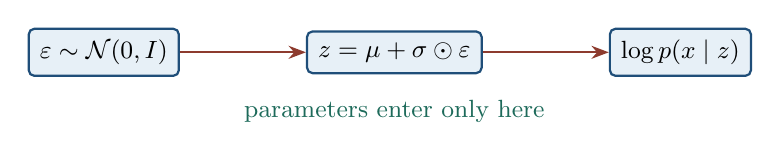
\begin{tikzpicture}[
  box/.style={draw=navy, thick, rounded corners=2pt, fill=navysoft, inner sep=4pt, font=\small},
  arr/.style={-{Stealth[length=2.2mm]}, thick, draw=burgundy}
]
\node[box] (eps) {$\varepsilon\sim\N(0,I)$};
\node[box, right=16mm of eps] (z) {$z=\mu+\sigma\odot\varepsilon$};
\node[box, right=16mm of z] (rec) {$\log p(x\given z)$};
\draw[arr] (eps) -- (z);
\draw[arr] (z) -- (rec);
\node[below=2mm of z, text=teal, font=\small] {parameters enter only here};
\end{tikzpicture}
\end{center}

For images in the notebook the decoder outputs Bernoulli logits, one per pixel. The reconstruction term is a binary cross-entropy with logits, summed over pixels and averaged over the batch. Do not apply a sigmoid before that loss. The sigmoid sits inside the stable implementation of the cross-entropy. With $\beta=1$ the training objective per image is that cross-entropy plus the KL in~\eqref{eq:stdkl}.

\begin{practbox}[Check the transform]
Let $\varepsilon\sim\N(0,1)$, $\mu=2$, $\sigma=3$. Find $\E[z]$ and $\mathrm{Var}(z)$ for $z=\mu+\sigma\varepsilon$. Then compute $\partial z/\partial\mu$ and $\partial z/\partial\sigma$.
\end{practbox}
\begin{solbox}
$\E[z]=2$ and $\mathrm{Var}(z)=9$, so $z\sim\N(2,9)$. The partial derivatives are $\partial z/\partial\mu=1$ and $\partial z/\partial\sigma=\varepsilon$. A loss $L(z)$ therefore has $\partial L/\partial\sigma=L'(z)\,\varepsilon$.
\end{solbox}

\chapter{Hierarchical latents}
\label{ch:hier}

One latent layer can be too weak a prior. A two-layer model draws a coarse code and then a fine code:
\[
p_\theta(x,z_1,z_2)=p_\theta(z_2)\,p_\theta(z_1\given z_2)\,p_\theta(x\given z_1),
\]
with the conditional independence $x\perp z_2\given z_1$. The variational family used in the homework respects the same order,
\[
q_\phi(z_1,z_2\given x)=q_\phi(z_2\given x)\,q_\phi(z_1\given z_2,x).
\]

\begin{center}
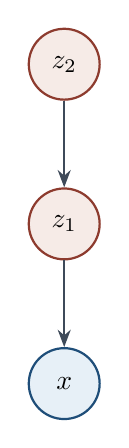
\begin{tikzpicture}[
  lat/.style={circle, draw=burgundy, thick, minimum size=9mm, fill=burgundysoft},
  obs/.style={circle, draw=navy, thick, minimum size=9mm, fill=navysoft},
  arr/.style={-{Stealth[length=2.2mm]}, thick, draw=slate}
]
\node[lat] (z2) {$z_2$};
\node[lat, below=11mm of z2] (z1) {$z_1$};
\node[obs, below=11mm of z1] (x) {$x$};
\draw[arr] (z2) -- (z1);
\draw[arr] (z1) -- (x);
\end{tikzpicture}
\end{center}

\section{The hierarchical ELBO}

Apply~\eqref{eq:elbokl} to the pair $(z_1,z_2)$. The gap is
\[
\log p_\theta(x)-\mathcal L_H(x)
=\KL\bigl(q(z_1,z_2\given x)\Vert p(z_1,z_2\given x)\bigr).
\]
Expand the joint and the variational factorizations. The cross terms separate into three pieces:
\begin{align*}
\mathcal L_H(x)
&=\E_{q(z_1,z_2\given x)}[\log p(x\given z_1)]
-\KL\bigl(q(z_2\given x)\Vert p(z_2)\bigr)\\
&\quad-\E_{q(z_2\given x)}\Bigl[\KL\bigl(q(z_1\given z_2,x)\Vert p(z_1\given z_2)\bigr)\Bigr].
\end{align*}
The inner KL is averaged under $q(z_2\given x)$ because $z_2$ is still random when that conditional KL is evaluated. You draw the coarse code from the approximate posterior, then score the fine code.

\section{Comparison with a one-layer bound}

Let $q(z_1\given x)$ be the marginal of the variational joint, and define the ordinary ELBO that uses only $z_1$,
\[
\mathcal L_M(x)
=\E_{q(z_1\given x)}[\log p(x\given z_1)]
-\KL\bigl(q(z_1\given x)\Vert p(z_1)\bigr).
\]
A second KL decomposition, this time of $q(z_2\given z_1,x)$ against $p(z_2\given z_1)$, yields
\[
\mathcal L_H(x)
=\mathcal L_M(x)
-\E_{q(z_1\given x)}\Bigl[\KL\bigl(q(z_2\given z_1,x)\Vert p(z_2\given z_1)\bigr)\Bigr].
\]
The subtracted term is nonnegative, so $\mathcal L_H\le\mathcal L_M$. Equality holds if and only if $q(z_2\given z_1,x)=p(z_2\given z_1)$ almost everywhere. For a fixed marginal $q(z_1\given x)$, that conditional is exactly the one that maximizes $\mathcal L_H$.

The marginal prior $p(z_1)=\int p(z_1\given z_2)p(z_2)\,dz_2$ may have no closed form. For an arbitrary positive auxiliary $r(z_2\given z_1)$,
\begin{align*}
\log p(z_1)
&=\E_{r}[\log p(z_1\given z_2)]-\KL(r(z_2\given z_1)\Vert p(z_2))\\
&\quad+\KL(r(z_2\given z_1)\Vert p(z_2\given z_1)).
\end{align*}
Drop the last KL, which is nonnegative, and you have a lower bound. The bound is an equality when $r=p(z_2\given z_1)$. Therefore
\[
\log p(z_1)
=\sup_r\Bigl\{\E_r[\log p(z_1\given z_2)]-\KL(r\Vert p(z_2))\Bigr\},
\]
and the supremum is attained at the true conditional. This is the same ``gap equals a KL'' pattern as~\eqref{eq:elbokl}.

\begin{practbox}
In the decomposition of $\mathcal L_H$, why is the fine-code KL inside an expectation over $q(z_2\given x)$, rather than evaluated at a single $z_2$?
\end{practbox}
\begin{solbox}
The KL $\KL(q(z_1\given z_2,x)\Vert p(z_1\given z_2))$ is a function of $z_2$. The variational joint draws $z_2$ from $q(z_2\given x)$ before drawing $z_1$. Taking the expectation is what the joint KL produces when you integrate that coordinate. Freezing one $z_2$ would describe a different, degenerate inference distribution.
\end{solbox}

\chapter{Normalizing flows}
\label{ch:flow}

\section{Change of variables as a model}

Choose a simple base $u\sim p_0=\N(0,I)$ and a stack of invertible maps $y=f(u)$. Equation~\eqref{eq:cov} gives the exact density of $y$. There is no ELBO. Training maximizes the log-density of the data, which is a base log-density plus a sum of log-absolute-determinants, one per layer. Lecture~5, slides~3--34, builds this from equivalent events up to the chain rule for Jacobians:
\[
\log\lvert\det J_{f_K\circ\cdots\circ f_1}\rvert
=\sum_{k=1}^K\log\lvert\det J_{f_k}\rvert.
\]

\begin{intbox}
A flow spends its capacity on maps whose Jacobian determinant is cheap. A generic neural network is invertible only by accident, and its determinant costs $O(D^3)$. Coupling layers, autoregressive maps, and $1\times 1$ convolutions are the designs that keep the determinant in closed form.
\end{intbox}

\section{Affine coupling}

Split $h=(h_A,h_B)$ with dimensions $d_A+d_B=D$. RealNVP, Lecture~5 slides~52--64, sets
\begin{align*}
y_A&=h_A,\\
y_B&=h_B\odot\exp\bigl(s(h_A)\bigr)+t(h_A).
\end{align*}
The functions $s$ and $t$ are ordinary neural networks. They need not be invertible.

\begin{resultbox}[Homework 2, problem 4.1]
The map is invertible:
\begin{align*}
h_A&=y_A,\\
h_B&=\bigl(y_B-t(y_A)\bigr)\odot\exp\bigl(-s(y_A)\bigr).
\end{align*}
Order the coordinates as $(A,B)$. The Jacobian is block triangular,
\[
J=\begin{pmatrix}I&0\\ \ast& \diag(e^{s(h_A)})\end{pmatrix},
\]
so $\log\lvert\det J\rvert=\sum_{j=1}^{d_B}s_j(h_A)$. Therefore
\[
\log p(y)=\log p_0(f^{-1}(y))-\sum_{j=1}^{d_B}s_j(y_A).
\]
The networks $s$ and $t$ do not appear in the determinant. Only the scale values do. That is why a large network is allowed.
\end{resultbox}

NICE is the special case $s\equiv 0$, an additive coupling. Then $\det J=1$. A separate diagonal rescaling layer carries the change of volume. Alternating which half is updated, and inserting a permutation of channels between couplings, lets every coordinate be transformed.

\begin{practbox}[Invert a $2$-D coupling by hand]
Let $s(h_1)=\log 2$ and $t(h_1)=h_1$. Forward-map $(h_1,h_2)=(1,3)$. Then invert the result.
\end{practbox}
\begin{solbox}
$y_1=1$ and $y_2=3\cdot e^{\log 2}+1=7$. The inverse reads $h_1=y_1=1$ and $h_2=(7-1)\cdot e^{-\log 2}=3$. The log-absolute-determinant of the forward map is $\log 2$.
\end{solbox}

\section{A flow as a VAE prior}

Keep a decoder $p_\theta(x\given z)$ and replace the prior by a flow. Draw $u\sim\N(0,I)$, set $z=f_\psi(u)$, and let $p_\psi$ be the induced density of $z$. The ELBO is still reconstruction minus a KL,
\[
\mathcal L_{\theta,\psi}(x)
=\E_{q(z\given x)}[\log p_\theta(x\given z)]
-\KL\bigl(q(z\given x)\Vert p_\psi(z)\bigr),
\]
and the change of variables writes the prior log-density as
\[
\log p_\psi(z)=\log p_0(f^{-1}(z))-\log\lvert\det J_f(f^{-1}(z))\rvert.
\]
Equivalently, define a decoder on the base space by $\tilde p(x\given u)=p(x\given f(u))$. Integrating $u$ against $p_0$ gives the same marginal $p(x)$ as integrating $z$ against $p_\psi$. If $z\sim q(z\given x)$ and $u=f^{-1}(z)$, the induced density is
\[
r(u\given x)=q(f(u)\given x)\,\lvert\det J_f(u)\rvert,
\]
and $\KL(q\Vert p_\psi)=\KL(r\Vert p_0)$. The two ELBOs agree when the variational densities are exact images of each other.

\begin{pitbox}[Where the equivalence dies]
Restrict both variational families to diagonal Gaussians. Take $f(u_1,u_2)=(u_1,u_2+u_1^2)$ and $q(z)=\N(0,I_2)$. Section~\ref{ch:calc} showed that $\det J_f=1$ and that the induced density of $u=f^{-1}(z)$ is
\[
r(u)\propto\exp\bigl(-\tfrac12 u_1^2-\tfrac12(u_2+u_1^2)^2\bigr),
\]
up to the constant of the standard normal. This is not a diagonal Gaussian: the coordinates are dependent. No diagonal-Gaussian encoder in $u$-space represents $r$. Optimizing over diagonal Gaussians in $z$ and in $u$ are different problems, even though the generative models are the same.
\end{pitbox}

\section{Masked autoregressive flows}

An autoregressive map with $y_d=\mu_d(y_{<d})+\sigma_d(y_{<d})\,\varepsilon_d$ is triangular. Its log-determinant is $\sum_d\log\sigma_d$. MADE masks evaluate every $\mu_d$ and $\sigma_d$ in one pass. Likelihood is parallel. Sampling remains sequential, because $y_d$ needs $y_{<d}$. That is Lecture~5, slides~65--73, and it is part~III of the flow notebook: a two-dimensional MAF on Lab chroma. An inverse autoregressive flow swaps the cost. Sampling becomes parallel and likelihood becomes sequential. The notebook asks for a MAF, not an IAF.

\section{From a density to a pixel probability}

A flow defines a density on $\R^D$. An image $x\in\Z^D$ is discrete. Assign to $x$ the bin $B_x=x+[0,1)^D$. These bins partition $\R^D$ up to boundaries of measure zero. If $y$ has density $p_\theta$ and $x=\lfloor y\rfloor$, then
\[
P_\theta(x)=\int_{[0,1)^D}p_\theta(x+u)\,du.
\]
Each value is nonnegative, and the sum over $x\in\Z^D$ equals $\int_{\R^D}p_\theta=1$. So $P_\theta$ is a probability mass function. The number $p_\theta(x)$ is a density evaluated at the corner of the bin. It is not $P_\theta(x)$.

The integral has no closed form for a neural flow. Choose a dequantizer $q(u\given x)$ supported on the unit bin, strictly positive inside it. Importance sampling writes
\[
P_\theta(x)=\E_{q(u\given x)}\Bigl[\frac{p_\theta(x+u)}{q(u\given x)}\Bigr].
\]
Jensen produces the variational dequantization bound
\begin{equation}
\label{eq:dq}
\log P_\theta(x)
\ge
\E_{q}\Bigl[\log\frac{p_\theta(x+u)}{q(u\given x)}\Bigr]
=\E_q[\log p_\theta(x+u)]+H\bigl(q(\cdot\given x)\bigr).
\end{equation}
The first term wants $x+u$ where the flow density is high. The entropy stops $q$ from collapsing to a point, which would throw away the integral.

Define the normalized restriction of the model to the bin,
\[
r_\theta(u\given x)=\frac{p_\theta(x+u)}{P_\theta(x)},\qquad u\in[0,1)^D.
\]
The same KL algebra as~\eqref{eq:elbokl} gives
\[
\log P_\theta(x)-\mathcal L_{\mathrm{DQ}}
=\KL\bigl(q(u\given x)\Vert r_\theta(u\given x)\bigr).
\]
The bound is tight if and only if $q=r_\theta(\cdot\given x)$.

Uniform dequantization sets $q=1$ on the bin. The bound becomes $\int_{[0,1)^D}\log p_\theta(x+u)\,du$, and it is tight if and only if $p_\theta(x+u)$ is constant on the bin. A conditional flow $u=g_\phi(\varepsilon;x)$, with $\varepsilon\sim p_0$ and $g_\phi(\cdot;x)$ a bijection onto $(0,1)^D$, substitutes the change-of-variables formula into~\eqref{eq:dq}:
\[
\mathcal L_{\mathrm{DQ}}
=\E_{\varepsilon}\Bigl[
\log p_\theta\bigl(x+g_\phi(\varepsilon;x)\bigr)
+\log\lvert\det J_{g}(\varepsilon;x)\rvert
-\log p_0(\varepsilon)
\Bigr].
\]
A learned $g$ can match a non-uniform $r$, so the KL gap can be smaller than the uniform gap.

\begin{center}
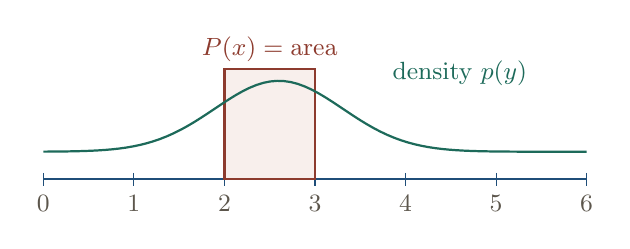
\begin{tikzpicture}[x=1.15cm,y=1cm]
  \draw[navy, thick] (0,0) -- (6,0);
  \foreach \x in {0,1,2,3,4,5,6} {\draw[navy] (\x,0.08) -- (\x,-0.08) node[below, text=muted, font=\small] {\x};}
  \draw[burgundy, thick, fill=burgundysoft, fill opacity=0.8] (2,0) rectangle (3,1.4);
  \node[burgundy, font=\small] at (2.5,1.65) {$P(x)=\mathrm{area}$};
  \draw[teal, thick, domain=0:6, samples=80] plot (\x,{0.35+0.9*exp(-(\x-2.6)*(\x-2.6))});
  \node[teal, font=\small] at (4.6,1.35) {density $p(y)$};
\end{tikzpicture}
\end{center}
\begin{center}
\textcolor{muted}{\small The probability of an integer is the area of the density over the unit bin, not the height of the density.}
\end{center}

\section{Invertible $1\times 1$ convolutions}

RealNVP mixes channels with a fixed permutation. Glow learns the mix. For a tensor $X\in\R^{C\times H\times W}$,
\[
Y_{:,i,j}=W X_{:,i,j},\qquad W\in\R^{C\times C},
\]
with the same $W$ at every spatial site.

\begin{resultbox}[Homework 2, problem 5]
The map is invertible if and only if $\det W\neq 0$, and the inverse applies $W^{-1}$ at each site. Vectorize the tensor in an order that keeps the $C$ channels of each pixel together. The full Jacobian is block diagonal with $HW$ blocks, each equal to $W$. Hence
\[
\log\lvert\det J\rvert=HW\log\lvert\det W\rvert.
\]
With the parameterization $W=PL\bigl(U+\diag(s)\bigr)$ of the previous determinant lemma,
\[
\log\lvert\det J\rvert=HW\sum_{i=1}^{C}\log\lvert s_i\rvert.
\]
The cost of the log-determinant is linear in the number of channels, not cubic, and it does not grow with a matrix factorization at every pixel.
\end{resultbox}

\begin{practbox}[One pixel, two channels]
Let $H=W=1$ and $W=\diag(2,1/2)$. Compute $\log\lvert\det J\rvert$ two ways: from $HW\log\lvert\det W\rvert$, and from the sum of $\log\lvert s_i\rvert$.
\end{practbox}
\begin{solbox}
$\det W=1$, so $\log\lvert\det J\rvert=0$. And $\log\lvert 2\rvert+\log\lvert 1/2\rvert=\log 2+\log(1/2)=0$. The volume of the two channels is unchanged: one axis stretches by $2$, the other shrinks by $2$.
\end{solbox}

\chapter{A short practice set}
\label{ch:set}

These five problems chain the moves above. Write the solution before you open the box.

\begin{practbox}[Set, problem A]
Let $q=\N(0,\diag(1,e))$ and $p=\N(0,I_2)$. Compute $\KL(q\Vert p)$ from~\eqref{eq:stdkl}.
\end{practbox}
\begin{solbox}
Coordinate $1$ contributes $0$. Coordinate $2$ has $\mu=0$ and $\sigma^2=e$, so $\tfrac12(e-1-\log e)=\tfrac12(e-2)$. The sum is $(e-2)/2$.
\end{solbox}

\begin{practbox}[Set, problem B]
Show that if $p(x\given z)=p(x)$ does not depend on $z$, and $q(z)=p(z)$, then the ELBO equals $\log p(x)$.
\end{practbox}
\begin{solbox}
The reconstruction term is $\E_q[\log p(x)]=\log p(x)$. The KL against the prior is zero. This is the collapsed case: the bound is tight because the latent was never used.
\end{solbox}

\begin{practbox}[Set, problem C]
Give the inverse and the log-absolute-determinant of $y_1=h_1$, $y_2=h_2 e^{h_1}+h_1^2$.
\end{practbox}
\begin{solbox}
$h_1=y_1$ and $h_2=(y_2-y_1^2)e^{-y_1}$. The Jacobian is triangular with diagonal $(1, e^{h_1})$, so the log-absolute-determinant is $h_1=y_1$.
\end{solbox}

\begin{practbox}[Set, problem D]
On the bin $[0,1)$, let $p(x+u)=c\,e^{u}$ for $u\in[0,1)$, with $c$ chosen so that you do not need its value. Is uniform dequantization tight?
\end{practbox}
\begin{solbox}
No. Tightness needs $p(x+u)$ constant in $u$. Here it grows with $u$. The optimal $q$ is proportional to $e^{u}$ on the bin.
\end{solbox}

\begin{practbox}[Set, problem E]
A $1\times 1$ convolution uses $W=\begin{psmallmatrix}0&1\\1&0\end{psmallmatrix}$ on a $3\times 4$ feature map with $2$ channels. Compute $\log\lvert\det J\rvert$.
\end{practbox}
\begin{solbox}
$W$ is a permutation, so $\lvert\det W\rvert=1$ and the log-determinant is zero. The spatial factor $HW=12$ multiplies zero. Permutations mix channels and do not change volume. Glow's learned diagonal $s$ is what changes volume.
\end{solbox}

\chapter*{References and slide index}
\addcontentsline{toc}{chapter}{References and slide index}

The lectures are the primary source. The books and papers below are the ones named on Lecture~0, slide~12, on Lecture~5, slide~84, and in the homework sheets.

\begin{itemize}[leftmargin=1.2em]
\item Sajjad Amini, Deep Generative Models lecture decks. Lecture~2, slides 12--42, for densities, expectation, Monte Carlo, and KL. Lecture~3 for autoregressive models and MADE. Lecture~4, slides 12--40, 56--64, and 77--84, for the ELBO and the reparameterization trick. Lecture~5, slides 3--73, for change of variables, NICE, RealNVP, and MAF.
\item Kevin P.\ Murphy, \emph{Probabilistic Machine Learning: Advanced Topics}, MIT Press, 2023. Chapter~10 for variational inference, Chapter~11 for Monte Carlo and importance sampling, Chapter~21 for variational autoencoders, Chapter~23 for normalizing flows.
\item Jakub M.\ Tomczak, \emph{Deep Generative Modeling}, Springer. Section~4.1.2 for the change of variables, \S4.1.3 for RealNVP and dequantization, \S5.3 for the VAE, \S5.3.6 for posterior collapse, \S5.4.1.4 for a mixture prior, \S5.4.1.8 for a flow prior, \S5.5.2.1 for a two-level hierarchical VAE.
\item Christopher M.\ Bishop and Hugh Bishop, \emph{Deep Learning: Foundations and Concepts}, Springer, 2023. The third book listed on the logistics slide.
\item D.\ P.\ Kingma and M.\ Welling, Auto-Encoding Variational Bayes, ICLR 2014.
\item D.\ P.\ Kingma and M.\ Welling, An Introduction to Variational Autoencoders, \emph{Foundations and Trends in Machine Learning}, 2019.
\item K.\ Sohn, H.\ Lee, and X.\ Yan, Learning Structured Output Representation using Deep Conditional Generative Models, NeurIPS 2015.
\item C.\ K.\ S{\o}nderby, T.\ Raiko, L.\ Maal{\o}e, S.\ K.\ S{\o}nderby, and O.\ Winther, Ladder Variational Autoencoders, NeurIPS 2016.
\item D.\ J.\ Rezende and S.\ Mohamed, Variational Inference with Normalizing Flows, ICML 2015.
\item L.\ Dinh, D.\ Krueger, and Y.\ Bengio, NICE: Non-linear Independent Components Estimation, 2015.
\item L.\ Dinh, J.\ Sohl-Dickstein, and S.\ Bengio, Density Estimation using Real NVP, ICLR 2017.
\item G.\ Papamakarios, T.\ Pavlakou, and I.\ Murray, Masked Autoregressive Flow for Density Estimation, NeurIPS 2017.
\item D.\ P.\ Kingma and P.\ Dhariwal, Glow: Generative Flow with Invertible $1\times 1$ Convolutions, NeurIPS 2018.
\item J.\ Ho, X.\ Chen, A.\ Srinivas, Y.\ Duan, and P.\ Abbeel, Flow++: Improving Flow-Based Generative Models with Variational Dequantization and Architecture Design, ICML 2019.
\item M.\ Germain, K.\ Gregor, I.\ Murray, and H.\ Larochelle, MADE: Masked Autoencoder for Distribution Estimation, ICML 2015.
\end{itemize}

\begin{intbox}[A path through the two homeworks]
Read Chapters~\ref{ch:prob}--\ref{ch:info} once. Do Homework~1's Gaussian and divergence problems from Chapters~\ref{ch:gauss} and~\ref{ch:mc}, and the autoregressive problems from Chapter~\ref{ch:ar}. Then read Chapter~\ref{ch:vae} and write the conditional ELBO before you train the VAE notebook. Read Chapter~\ref{ch:hier} before problem~2. Read the coupling section of Chapter~\ref{ch:flow} before problems~3, 4, and~5, and before the flow notebook. Do the notebook's color-transfer section first. It is the two-dimensional MAF.
\end{intbox}

\end{document}
